%version of 08-14-19

\chapter{Recurrences:
Rendering Complex Structures Manageable}
\label{ch:Recurrences}

One of the intellectually most powerful strategies for all manner of
human endeavor is to ``learn from the past''---i.e., to {\em re}-use
knowledge that one has acquired earlier in order to acquire new
knowledge.  Within the domain of computing, this strategy is
exemplified by computations that derive the value of a function $F$ at
an argument $n \in \N^+$ by invoking the (hopefully, earlier-computed)
values of $F$ at arguments $1, 2, \ldots, n-1$.  The classical first
example of such a {\it recurrent} mode of computing involves the {\it
  factorial function} {\sc Fact} of Section~\ref{sec:unary-ops}.C.
\index{arithmetic!basic operations!factorial (of a nonnegative integer)}
The ``direct'' mode of computing {\sc Fact} at an argument $n \in
\N^+$ is:
\[ \mbox{\sc Fact}(n) \ = \ 1 \times 2 \times \cdots \times n. \]
The {\em recurrent} mode of computing {\sc Fact}($n$) is more
compact---and it better exposes the inherent structure of the
function.
\[ \mbox{\sc Fact}(n) \ = \ \left\{
\begin{array}{cl}
 n \times \mbox{\sc Fact}(n-1) & \mbox{ if } \ n > 1 \\
 1 & \mbox{ if } \ n = 1 \\
\end{array}
\right.
\]
This chapter is devoted to deriving and solving a variety of types of
recurrences.  In common with the rest of this text, our treatment of
this subject emphasizes exploiting recurrent structure in reasoning
and analysis: increased understanding will enable improved computing.


\section{Linear Recurrences}
\label{sec:linear-recurrences}
\index{linear recurrences}

This section is devoted to the solution of {\em linear} recurrences,
as exemplified by the following function specifications, wherein $a$,
$b$, $c$, and $d$ are integers

%{\Denis Should we change the notation of F here? since it will be used for Fibo elements in the following section of the chapter. We can keep it as it is, and add a note about the abstract letters usually $x$ for any variable and $F$ for any function...}
%{\Denis I changed the bounds in the expression to keep more generality.
%I also changed f(1) for a constant c replacing 1}
%{\Denis We should say here that $a$, $b$ and $c$ are integers}

\newpage

\begin{eqnarray}
\nonumber
\mbox{\bf The general form} & & \\
\label{eq:Lin-Recur:general}
f(n) & = & \left\{
\begin{array}{cl}
a f(n/b) + g(n) & \hspace*{.2in} \mbox{for } n \geq b \\
c & \hspace*{.2in} \mbox{for } n < b
\end{array}
\right. \\
\nonumber
  & & \\
\nonumber
\mbox{\bf The simple form} & & \\
\label{eq:Lin-Recur:basic}
f(n) & = & \left\{
\begin{array}{cl}
a f(n/b) + d & \hspace*{.4in} \mbox{for } n \geq b \\
1 & \hspace*{.4in} \mbox{for } n < b
\end{array}
\right.
\end{eqnarray}

%{\Denis constant c ws used twice, this was a bit confuseing... Thus, I changed here f(1) to 1 since it is the simplified form...}

Myriad basic algorithmic problems, including sorting, selection,
matching, and more, can be solved using linear-recurrent
algorithms \cite{CLRS}---and such algorithms yield to specification
and analysis via linear recurrences.

In the next two subsections, we present analyses of recurrences
(\ref{eq:Lin-Recur:general}) and (\ref{eq:Lin-Recur:basic}).  The
reader will be able to extend the techniques we use in our analyses of
these specific recurrences in order to analyze other members of the
important family of linear-recurrent algorithms.


\subsection{The Master Theorem for the Simple Linear Recurrence} 
\label{sec:masterTheorem}
\label{sec:linear-recurrence-basic}

We focus first on the simpler of our sample recurrences, namely,
(\ref{eq:Lin-Recur:basic}).  Happily, there is a single perspicuous
proof that elegantly solves recurrences of this form.

By the time the reader has reached this paragraph, she has the
mathematical tools necessary to prove and apply what is called {\it
  The Master Theorem for Linear Recurrences} \cite{CLRS}.  The main
tools in the proof of the Theorem are: summing geometric summations
(Section~\ref{sec:geometric-sums}) and employing elementary asymptotic
notions and notations (Section~\ref{sec:asymptotics}).

\begin{theorem}[The Master Theorem for the simple linear recurrence]
\label{thm:master-thm-simple}
\index{The Master Theorem!for the simple linear recurrence}
Let the function $f$ be specified by the simple linear recurrence
(\ref{eq:Lin-Recur:basic}).  Then the value of $f$ on any argument $n$
is given by
\begin{equation}
\label{eq:Lin-Recur:solve}
\begin{array}{lcllll}
f(n) & = & (1 + \log_b n) \cdot c &  &  & \mbox{if } a=1 \\
     &   &                 &  &  & \\
     & = &
  {\displaystyle
  \frac{1-a^{\log_b n}}{1-a} \cdot c \ \ \approx \ \ \frac{c}{1-a}
  }
                           &  &  & \mbox{if } a<1 \\
    &   &                  &  &  & \\
    & = &
  {\displaystyle
\frac{a^{\log_b n} -1}{a-1} \cdot c
  }
                           &  &  & \mbox{if } a>1
\end{array}
\end{equation}
\end{theorem}

\begin{proof}
We expose the pattern generated by recurrence
(\ref{eq:Lin-Recur:basic}), by beginning to ``expand'' the specified
computation---replacing occurrences of $f(\bullet)$ as mandated in
(\ref{eq:Lin-Recur:basic}).  Once we discern the pattern, we jump to
the general form.
\begin{equation}
\label{eq:Lin-Recur:expand}
\begin{array}{lcccc}
f(n) & = & a f(n/b) + c & & \\
     & = & a \left( a f(n/b^2) + c \right) + c
             & = & a^2 f(n/b^2) + (a+1)c \\
     & = & a^2 \left( a f(n/b^3) + c \right) + (a+1)c
             & = & a^3 f(n/b^3) + (a^2+a+1)c \\
     &   & \vdots & & \vdots \\
     & = & 
{\displaystyle
\left(a^{\log_b n} + \cdots +a^2+a+1 \right) c
} & &
\end{array}
\end{equation}
The segment of (\ref{eq:Lin-Recur:expand}) ``hidden'' by the vertical
dots betokens an induction that is left to the reader.  Equations
(\ref{eq:geom-sum:b>1}) and (\ref{eq:geom-sum:b<1}) now enable us to
demonstrate that (\ref{eq:Lin-Recur:solve}) is the asserted
case-structured solution to (\ref{eq:Lin-Recur:basic}).  \qed
\end{proof}


\subsection{The Master Theorem for the General Linear Recurrence} 
\label{sec:linear-recurrence-general}

We now progress from the simple recurrence (\ref{eq:Lin-Recur:basic}) to
the more general recurrence (\ref{eq:Lin-Recur:general}).  We simplify
our problem in two ways, in order to avoid calculational complications
(such as floors and ceilings) that can mask the principles that govern
our analysis.
\begin{enumerate}
\item
We employ a very simple nonrecurrent function $g$: We focus on the
case $g(n) = n$.

It requires only clerical effort to generalize to the slightly more
ambitious $g(n) = \alpha n + \beta$ (so that $g$ is a general {\em
  linear} function), but such an extension teaches no new lessons.
\item
We assume that the argument $n$ to functions $f$ and $g$ is a power of
$b$.

This allows us to concentrate on the general unfolding of the
recurrence without worrying about floors and ceilings.

\item We consider $c=1$.
\end{enumerate}
Removing these assumptions would significantly complicate our
calculations, but it would not change our reasoning.

\begin{theorem}[The Master Theorem for the general linear recurrence]
\label{thm:master-thm-genl}
\index{The Master Theorem!for the general linear recurrence}
Let the function $f$ be specified by the general linear recurrence
(\ref{eq:Lin-Recur:general}).  Then the value of $f$ on any argument
$n$ is given by
\[
f(n) \ = \ 
a^{\log_b n} f(1) \ \ + \ \ \left( \sum_{i=0}^{\log_b (n)-1} (a/b)^i \right) n
\]

\noindent
When $a > b$, the behavior of $f(n)$ is dominated by the first
term of this solution:
\[ a^{\log_b n} \cdot  f(1) \ \ = \ \ n^{\log_b a} \]

\noindent
When $a < b$, the behavior of $f(n)$ is dominated by the second
term of this solution:
\[
n \cdot \sum_{i=0}^{\log_b (n)-1} (a/b)^i
  \ \ = \ \
\frac{\left( 1 \ - \  (a/b)^{\log_b (n)} \right)}{1- (a/b)} \cdot n \ \
  \ \ \approx \ \
\frac{b}{b - a} \cdot n
\]
\end{theorem}

\begin{proof}
As in Section~\ref{sec:linear-recurrence-basic}, we expose the
algebraic pattern created by the recurrence ``unfolding''
(\ref{eq:Lin-Recur:general}).  As in (\ref{eq:Lin-Recur:expand}), once
we discern this pattern, we jump to the general form (which can be
verified via induction).
\[
\begin{array}{ccccc}
f(n) & = & a f(n/b) + n & & \\
     & = & a \left( a f(n/b^2) + n/b \right) + n
             & = & a^2 f(n/b^2) + (an/b+n) \\
     & = & a^2 \left( a f(n/b^3) + n/b^2 \right) + (a/b+1)n
             & = & a^3 f(n/b^3) + (a^2/b^2+a/b+1)n \\
     &   & \vdots & & \vdots \\
    & = & 
{\displaystyle
a^{\log_b n} f(1) + \left( \sum_{i=0}^{\log_b (n)-1} (a/b)^i \right) n
} & &
\end{array}
\]

We thus see that solving the more general recurrence
(\ref{eq:Lin-Recur:general}) requires only augmenting the solution to
the simple recurrence (\ref{eq:Lin-Recur:basic}) by ``appending'' to
the simple solution a geometric summation whose base is the ratio
$a/b$.  The reader can now invoke the techniques from
Section~\ref{sec:summing-geometric-series:techniques} to arrive at the
announced solution to (\ref{eq:Lin-Recur:general}).

When one ``does'' mathematics, one is often interested in uncovering
the {\em dominant behavior} of the function $f(n)$ specified via a
recurrence such as (\ref{eq:Lin-Recur:general}).  Therefore, the two
assertions in the statement of the proposition, about the ``dominant''
behavior of function $f$ for given relative sizes of $a$ and $b$ is an
integral part of the lessons that we learn from this proof.

\ignore{*********
An important lesson
to garner from the analysis we have been performing throughout this
section is the following:
\begin{itemize}
\item
When $a > b$, the behavior of $f(n)$ is dominated by the first
term of the solution:
\[ a^{\log_b n} \cdot  f(1) \ \ = \ \ n^{\log_b a} \]

%{\Denis as we assumed f(1)=1, I remove f(1) in the last term}
\item
When $a < b$, the behavior of $f(n)$ is dominated by the second
term of the solution:
\begin{eqnarray*}
n \cdot \sum_{i=0}^{\log_b (n)-1} (a/b)^i
  & = &
\frac{\left( 1 \ - \  (a/b)^{\log_b (n)} \right)}{1-\frac{a}{b}} n \\
%  & = &
%n \ - \ a^{\log_b n} \\
  & \approx &
n \frac{b}{b - a}
\end{eqnarray*}
\end{itemize}

%{\Denis Is there a reason to avoid to write the theorem here as in the previous section?}
*********}


One can learn yet other lessons about $f(n)$, specifically about how
to compute $f(n)$ (exactly or approximately) by studying
Fig.~\ref{fig:masterTheorem}.
\begin{figure}[htb]
\begin{center}
       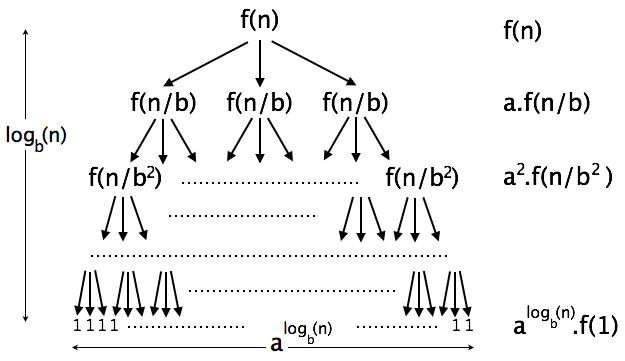
\includegraphics[scale=0.4]{FiguresMaths/MasterTheoremgeneral}
\caption{Development of the calculation specified by recurrence
  (\ref{eq:Lin-Recur:general}).  The total cost is obtained by the summation on each row:
  $a \times f(n/b)$ in the first row, $a^2 \times f(n/b^2)$ in the second row, and so on.
  This leads to $a^{log_b(n)}$.
\label{fig:masterTheorem}}
\end{center}
\end{figure}
In particular, one observes in the figure that when $a=b$, the
computations in each row are perfectly balanced.  When $a=b=2$, for
instance, the tree has $n$ leaves, and the computations inside the
tree evaluate to exactly $n$ at each of the tree's $ \ln(n)$
levels---so that $f(n) = n \ln(n)$ in this case.  \qed
\end{proof}
%{\Arny The notation in Fig.~\ref{fig:masterTheorem} (fonts, cdots) should be made consistent with the text.}


\subsection{An Important Application: Beginning Information Theory}
\label{sec:count-strings}

By the mid-$20$th century, the existence of electrical and electronic
devices that enhanced our ability to compute and to intercommunicate,
made it imperative that ``the experts'' understand the mathematical
laws that govern these activities.  In 1948, the American
mathematician and engineer Claude E.~Shannon
\index{Shannon, Claude E.}
revolutionized our understanding of these laws by inventing the field
of {\it information theory} \index{information theory}
\cite{Shannon48}.  Shannon's innovations enabled us to quantify the
quality of our handling of data: speed of transmission, efficiency of
encoding, vulnerability to errors.  The evolution of data science
\index{data science} and the ever-increasing importance of
information-related topics such as {\it encryption} and {\it data
  security} \index{data encryption} and \index{data security} make it
important that everyone who has contact with the world of computing
and communication---which means pretty much everyone---understand at
least the rudiments of information theory.  This section is devoted to
taking one small step in that direction, a step that hints at the
fundamental role that logarithms play in the theory. 

One of the most basic results within information theory highlights the
role of logarithms in measuring ``the amount of information'' that a
string can hold.

\begin{prop}
\label{thm:bound-stringnames-lgth-k}
Say that one must assign distinct labels to $n$ items, via strings
over an alphabet of $a$ symbols.  Then at least one string-label must
have length no shorter than $\lceil \log_a n \rceil$.
\end{prop}

\begin{proof}
Let $A$ be an alphabet of $a$ symbols.  For each integer $k \geq 0$,
let $A^{(k)}$ denote the set of all length-$k$ strings over $A$; note
that $A^{(1)} = A$.  The bound of
Proposition~\ref{thm:bound-stringnames-lgth-k} follows by counting the
numbers of strings of various lengths over $A$, because each such
string can label at most one item.  Let us, therefore, inductively
evaluate the cardinality $|A^{(k)}|$ of each set $A^{(k)}$.
\begin{itemize}
\item
$|A^{(0)}| =1$

This is because the null-string, commonly denoted $\varepsilon$, 
\index{null string $\varepsilon$}
\index{$\varepsilon$: the null string, of length $0$}
is the unique string in $A^{(0)}$; symbolically, $A^{(0)} = \{
\varepsilon \}$.

\item
$|A^{(k+1)}| = |A| \cdot |A^{(k)}|$.

This reckoning follows from the following recipe for creating all
strings of length $k+1$ from all strings of length $k$.
\[
A^{(k+1)} \ = \ \{ \sigma x \ | \ \sigma \in A \ \ \mbox{
  and } \ \ x \in A^{(k)} \}
\]
In other words, every length-$(k+1)$ string over $A$ is obtained
by taking a length-$k$ string $x$ over $A$ and {\em prepending}
\index{prepend a symbol to a string} to it a symbol from $A$.

This recipe is correct because
  \begin{itemize}
  \item
Each string in $A^{(k+1)}$, as constructed, has length $k+1$.

This is because the recipe adds a single symbol to a length-$k$
string.
  \item
For each string $x \in A^{(k)}$, there are $|A|$ distinct
strings in $A^{(k+1)}$, as constructed.

This is because each string in $A^{(k+1)}$ begins with a distinct
symbol from $A$.

  \item
$A^{(k+1)}$, as constructed, contains all strings of length $k+1$
over $A$.

This is because for each $\sigma \in A$ and each $x \in
A^{(k)}$, the string $\sigma x$ is in $A^{(k+1)}$, as
constructed.
  \end{itemize}
\end{itemize}
We thus have the following recurrence.
\begin{eqnarray*}
|A^{(0)}| & = & 1 \\
|A^{(k+1)}| & = & |A| \times |A^{(k)}| \ \ \ \ 
\mbox{ for } \ k \geq 0
\end{eqnarray*}
Theorem~\ref{thm:master-thm-simple} tells us that, for each $\ell \in \N$,
\[ |A^{(\ell)}| \ \ = \ \ \frac{|A|^{\ell+1} \ - \ |A|}
{|A| -1} \ \ \leq \ \ c' \cdot |A|^{\ell}
\]
for some constant $c'$.  In order for this quantity to reach the value
$n$, we must have
\[ \ell \ > \ d' \cdot \log_{|A|} n   \]
for some small constant $d'$.  \qed
\end{proof}

The following result can be considered anther way of looking at
Proposition~\ref{thm:bound-stringnames-lgth-k}.

\begin{prop}
\label{thm:Num-strings-lgth-k}
The number of distinct strings of length $k$ over an alphabet of $a$
symbols is $a^k$.
\end{prop}

\begin{proof}
As in Proposition~\ref{thm:bound-stringnames-lgth-k}, let us focus on
the generic $a$-letter alphabet $A \ = \ \{\sigma_1, \sigma_2,
\ldots, \sigma_a\}$.  We argue by induction on string-length $k$.

\noindent
{\it Bases.}
The induction we develop can start either with the unique string of
length $k=0$ or with strings of length $k=1$.  In the former case, the
uniqueness of the null string validates the case $k=0$ of the
proposition.  In the latter case, there are $a^1 = a$ such strings
over $A$, one for each symbol $\sigma \in A$; this validates the case
$k=1$ of the proposition.

\noindent
{\it The inductive hypothesis.}
Say that for all string-lengths $k$ up through $n$, there are $a^k$
distinct words of length $k$ over $A$.

\noindent
{\it Extending the induction.}
Take each length-$n$ string $x$ over $A$, and {\em append}
\index{append a symbol to a string} to it, in turn, each of $A$'s $a$
symbols, i.e., add each symbol to $x$ as an additional rightmost
symbol.  One thereby creates $a$ new strings, each obviously distinct,
for each string in $A^{(n)}$,: namely, $x \sigma_1$, $x \sigma_2$,
\ldots, $x \sigma_a$.  We have thus created $a^{n+1}$ distinct
length-$(n+1)$ strings over $A$ from $A$'s $a^n$ distinct length-$n$
strings.

The induction is thus extended, which completes the proof.  \qed
\end{proof}


\section{Bilinear Recurrences}
\label{sec:bilinear-recurrences}
\index{bilinear recurrences}

\subsection{Binomial Coefficients and Pascal's Triangle}
\label{sec:binomial-coeff+Pascal}

In Section~\ref{sec:binomial-coeff}, we introduced and briefly
discussed the binomial coefficient \index{binomial coefficients}
$\displaystyle \Delta_{n,k} \ \eqdef \ {n \choose k}$ in its guise as a
binary operation on integers; see (\ref{eq:binom-coeff}).  And, we
established in Proposition~\ref{thm:manipulate-binom-coeff} the
summation rule
\[ {n \choose k} \ + \ {n \choose {k+1}} \ = \ {{n+1} \choose {k+1}} \]
for $\Delta_{n,k}$.  In fact, one can {\em define} binomial
coefficient via the {\em bilinear recurrence} that underlies this
rule.  This change in viewpoint is the topic of the current
subsection.

\subsubsection{The formation rule for Pascal's Triangle}
\label{sec:Pascal-formation}

Let us define the bivariate integer function\footnote{We alter our
  notation for binomial coefficients in deference to our change in
  viewpoint: We promote the integer pair $\langle n,k \rangle$ from a
  subscript to an argument, and we embellish $\Delta$ with a
  hat.}~$\hat{\Delta}(n,k)$ via the bilinear recurrence
\begin{equation}
\label{eq:binom-coeff-recurrence}
\hat{\Delta}(n,k) \ = \ 
\left\{
\begin{array}{cl}
1  & \mbox{ if } \ [n=1, k=0] \\
1  & \mbox{ if } \ [n=1, k=1] \\
\hat{\Delta}(n-1, k-1) \ + \  \hat{\Delta}(n-1,k) & \mbox{ otherwise}
\end{array}
\right.
\end{equation}

\smallskip

We claim that the function $\hat{\Delta}(n,k)$ thus defined is, in
fact, the for binomial coefficient $\displaystyle {n \choose k}$.  We
establish this claim with the help of a two-dimensional array of
integers known as {\it Pascal's Triangle},
\index{Pascal's triangle}
so named in honor of the French polymath Blaise Pascal.
\index{Pascal, Blaise}
Fig.~\ref{fig:pascal-triangle} provides a ``prefix'' of this famed
array, for $n,k \leq 5$.
\begin{figure}[htb]
\[
\begin{array}{c||r|r|r|r|r|r|r|r|r|r|r}
{\displaystyle {n \choose k}} & k=0 & k=1 & k=2 & k=3 & k=4 & k=5 &
k=6 & k=7 & k=8 & k=9 & \ldots \\
\hline
\hline
n=1 & 1 & 1 &    &    &     &     &    &    &   &   & \ldots \\
\hline
n=2 & 1 & 2 &  1 &    &     &     &    &    &   &   & \ldots \\
\hline
n=3 & 1 & 3 &  3 &  1 &     &     &    &    &   &   & \ldots \\
\hline
n=4 & 1 & 4 &  6 &  4 &   1 &     &    &    &   &   & \ldots \\
\hline
n=5 & 1 & 5 & 10 & 10 &   5 &   1 &    &    &   &   & \ldots \\
\hline
n=6 & 1 & 6 & 15 & 20 &  15 &   6 &  1 &    &   &   & \ldots \\
\hline
n=7 & 1 & 7 & 21 & 35 &  35 &  21 &  7 &  1 &   &   & \ldots \\
\hline
n=8 & 1 & 8 & 28 & 56 &  70 &  56 & 28 &  8 & 1 &   & \ldots \\
\hline
n=9 & 1 & 9 & 36 & 84 & 126 & 126 & 84 & 36 & 9 & 1 & \ldots \\
\hline
\vdots &\vdots &\vdots &\vdots &\vdots &\vdots &\vdots &\vdots &\vdots
&\vdots &\vdots &\ddots
\end{array}
\] 
\caption{A ``prefix'' of Pascal's Triangle, for $n,k \leq 9$.}
\label{fig:pascal-triangle}
\end{figure}
The {\em formation rule of the array} is that the array-entry at (row
$n+1$, column $k+1$) is the sum of the array-entries at (row $n$, column
$k$) and at (row $n$, column $k+1$).
\index{Pascal's Triangle!formation rule}

\medskip

By comparing the formation rule for Pascal's Triangle with equation
(\ref{eq:add-binom-coeff}), you can anticipate the following result.

\begin{prop}
\label{thm:pascal-binom}
The entries of Pascal's Triangle are the binomial coefficients.
Specifically, for all $n,k$, the entry at (row $n$, column $k$) of the
Triangle is $\displaystyle {n \choose k}$.
\end{prop}

\begin{proof}
We note by observation and direct calculation (see
Fig.~\ref{fig:pascal-triangle}) that the proposition is true for $n =
1$ and $k \in \{0, 1\}$.  A simple double induction verifies that
every binomial coefficient appears in the Triangle and every Triangle
entry is a binomial coefficient.  \qed
\end{proof}

\ignore{****************** \\
induction on $n$, then for each value of $n$ on $k \leq n$ \\
{\Arny SHOULD WE SPELL THIS OUT IN DETAIL?  GIVE AS AN EXERCISE?} \\
{\Denis Yes, I think we can detail the classical recurrence proof. I added an alternative proof based on counting the number of paths in the Pascal's triangle -- see figure}
******************}

\begin{figure}[htb]
\begin{center}
       \includegraphics[scale=0.4]{FiguresMaths/CoeffBinomiaux1}
\caption{Another representation of the Pascal's triangle}.
\label{fig:binomialCoeff1}
\end{center}
\end{figure}

\begin{figure}[htb]
\begin{center}
       \includegraphics[scale=0.4]{FiguresMaths/CoeffBinomiaux2}
\caption{Argument for an alternative proof where the coefficient in row $n+1$ is obtained by the two previous coefficients in row $n$.
Then, the number of paths to reach this coefficient is equal to the sum of the number of paths in these two coefficients of the previous row.}
\label{fig:binomialCoeff2}
\end{center}
\end{figure}

\begin{figure}[htb]
\begin{center}
       \includegraphics[scale=0.4]{FiguresMaths/CoeffBinomiauxCounting}
\caption{There are three different paths for reaching ${3 \choose 2}.$}
\label{fig:binomialCoeff3}
\end{center}
\end{figure}

As an immediate consequence of the relation between binomial
coefficients and Pascal's Triangle, we observe the following {\it a
  priori} nonobvious fact.

\begin{prop}
\label{thm:binomcoeff-integer}
Every binomial coefficient is an integer.
\end{prop}
\index{binomial coefficients!integer-hood}

\begin{proof}
By the formation rule for Pascal's Triangle, every entry in that array
is obtained from integers via repeated additions.  The present result
therefore follows from Proposition~\ref{thm:pascal-binom}'s proof that
the elements of the Triangle are precisely the binomial coefficients.  \qed
\end{proof}


\subsubsection{The summation formula for binomial coefficients}
\label{sec:summaion-BinCoeff}

We conclude this section with a very consequential result about the
binomial coefficients.  We shall observe applications of this result
as we explore a variety of topics, ranging from counting discrete
structures and calculating probabilities to deriving basic properties
of other recursively defined families.


\begin{prop}
\label{thm:sumsof-binomcoeff}
For every positive integer $n$,
\[
\sum_{i=0}^n \ {n \choose i} \ \ = \ \
{n \choose 0} \ + \ {n \choose 1} \ + \cdots + \ {n \choose {n-1}} \ +
\ {n \choose n} \ \ = \ \ 2^n
\]
\end{prop}
\index{binomial coefficients!summation formula}

\begin{proof}
This result is an immediate consequence of the Binomial Theorem
(Theorem~\ref{thm:Binomial-theorem}).  That seminal result tells us
that, for all $n \in \N$,
\[
(x+y)^n \ \ = \ \ \sum_{i=0}^n \ \ {n \choose i} x^{n-i} y^i
\]
If we instantiate this polynomial equation with the values $x = y =
1$, then we obtain the present result.
\qed
\end{proof}


\subsection{The Fibonacci Number Sequence}
\label{sec:Fibonacci}
\index{Fibonacci sequence}
\index{Fibonacci numbers}

This section is devoted to one of the most storied topics in the world
of mathematics---in terms of the topic's manifestation in the real
world and in terms of the multiple names used to refer to its
discoverer,\footnote{Not surprisingly, this marvelous sequence was
  discovered many times, in many places.  Our story refers ony to its
  discovery in the West.}~the 13th-century Italian mathematician
variously known as: \index{Fibonacci, Leonardo}
\index{Fibonacci, Leonardo!alternative names}

\begin{tabular}{ll}
Fibonacci               & (abbreviated Italian for: son of Bonaccio) \\
Leonardo of Pisa        & (his hometown) \\
Leonardo Pisano         & (variant of ``of Pisa'') \\
Leonardo Pisano Bigolo  & (his hometown plus family name) \\
Leonardo Fibonacci      & (for: son of Bonaccio Bigolo) \\
Leonardo Bonacci        & (for: son of Bonaccio Bigolo) \\
\end{tabular}

\medskip

\noindent
The sequence discovered by this multi-named genius is defined as follows.

\medskip

The {\it Fibonacci sequence}, or, {\it the Fibonacci numbers}, is an
infinite sequence
\[ F(0), \ F(1), \ F(2), \ \ldots \]
of elements of $\N^+$, the set of positive integers.  As just denoted,
we see that the numbers in the sequence are traditionally indexed by
elements of $\N$, the set of nonnegative integers and are often
written using functional ($F(i)$) notation rather than subscripts
($F_i$).  The classical definition of the sequence is as follows.
\index{Fibonacci sequence!definition}\index{Fibonacci numbers!definition}
\begin{eqnarray}
\nonumber
F(0) & = & 1 \\
\label{eq:Fibonacci-defn}
F(1) & = & 1 \\
\nonumber
F(n) & = & F(n-1) \ + \ F(n-2) \ \ \ \mbox{ for all } n > 1
\end{eqnarray}
The sequence is often specified just by listing its early elements:
\[ 1, \ 1, \ 2, \ 3, \ 5, \ 8, \ 13, \ 21, \ 34, \ \ldots \]


\subsubsection{The story of the Fibonacci numbers}
\label{sec:Fibonacci-story}
\index{Fibonacci sequence!story}
\index{Fibonacci numbers!story}

Leonardo Fibonnaci describes\footnote{In his {\it Liber Abaci}}
discovering his eponymous sequence in the course of contemplating the
rate of population growth of successive generations of an idealized
immortal initial pair of rabbits.  Rabbits mature quickly and, after
attaining maturity at one month, can spawn a new pair of progeny every
following month.  So, at ``time $0$'', there is one pair of rabbits.
This persists at month $1$, because there has not yet been time to
produce new rabbits.  By month $2$, though, there are $2$ pairs of
rabbits.  At month $3$, only the first pair will have spawned, so
there are $3$ pairs of rabbits.  At month $4$, these $3$ pairs are
joined by $2$ more.  The reader can continue this story and discover
that the number of pairs of rabbits observed after successive months
are given by the sequence generated by the process implicit in
recurrence (\ref{eq:Fibonacci-defn}) and illustrated by our initial list.
Fig.~\ref{fig:fibo5} below illustrates the process up to month $4$.
\begin{figure}[htb]
\begin{center}
        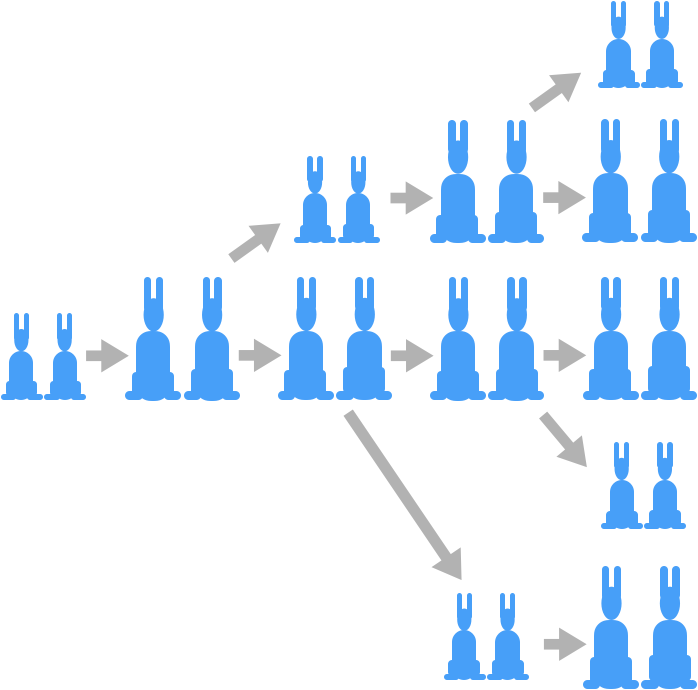
\includegraphics[scale=0.3]{FiguresMaths//Fibo5}
\caption{The successive generations of rabbits are growing each month
  (depicted for the first four months).}
        \label{fig:fibo5}
\end{center}
\end{figure}

The Fibonacci sequence's role in describing idealized rabbit
population statistics is no more fascinating than its appearance
elsewhere in the natural world---in structural features such as the
patterns of seeds in flower heads, the numbers of petals of flowers,
the growth patterns of pine cones and pineapples, and on and on; see
\cite{Basin63}.

The story of this fascinating sequence of numbers has a macroscopic
aspect also.  Many cultures, the ancient Greeks among them, have
attributed mystical properties to (classes of) numbers; our
discussions about the {\it prime numbers} in Section~\ref{sec:primes}
and about the {\it perfect numbers} in
Section~\ref{sec:perfect-numbers+Mersenne-primes} bear witness to this
phenomenon.  One specific number that has attracted such attention is
the {\it golden ratio}, an irrational real number which is usually
denoted $\Phi$ and which has the following (exact and approximate)
values: \index{golden ratio, $\Phi$} \index{$\Phi$, the golden ratio}
\[ \Phi \ = \ \frac{1+\sqrt{5}}{2} \ \approx \  1.618\ldots \]
It has been alleged that rectangles whose {\it aspect ratios} (Length
$\div$ Width) are (roughly) $\Phi$ are the most pleasing to the human
eye.  In fact, the aspect ratio of the Parthenon, in Athens is
(roughly) $\Phi$, although it is not known whether this is
intentional.  The relevance of $\Phi$ to this section resides in the
fact that {\em the sequence of ratios of successive Fibonacci numbers
approaches $\Phi$}.

You can perform your own test about pleasing rectangles and ratios of
successive Fibonacci numbers by perusing Fig.~\ref{fig:fibosquare}.
\begin{figure}[htb]
\begin{center}
        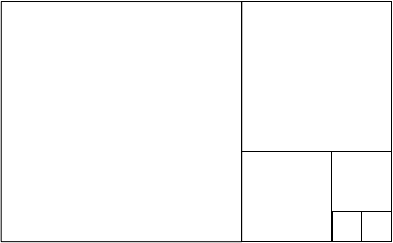
\includegraphics[scale=0.5]{FiguresMaths//Fiboembedded}
\caption{Successive Fibonacci numbers interpreted geometrically, via a
  spiral of squares whose respective sides form a Fibonacci
  sequence.}
        \label{fig:fibosquare}
\end{center}
\end{figure}

The mathematical properties of this truly remarkable sequence will
occupy our attention in the remainder of this section.


\subsubsection{Fibonacci numbers and binomial coefficients}
\label{sec:FibNo+BinomCoeff}
\index{Fibonacci numbers!connection with binomial coefficients}
\index{binomial coefficients!connection with Fibonacci numbers}

%\begin{figure}[h]
%\begin{center}
%        \includegraphics[scale=0.4]{FIGmaths/DefFibo}
%        \caption{Principle of the Fibonacci progression}
%        \label{doublesum}
%\end{center}
%\end{figure}
%Notice that it is a special case of $u_{n+1} =\alpha.u_{n} + \beta.u_{n-1}$ for $\alpha=\beta=1$.
%\bigskip

There is a strong, nonobvious, connection between the binomial
coefficients of Section~\ref{sec:binomial-coeff+Pascal} and the
Fibonacci numbers of the current section.  We observe this connection
by contemplating the diagonals of Pascal's Triangle.  See
Fig.~\ref{fig:FiboPascal}.
\begin{figure}[htb]
\begin{center}
        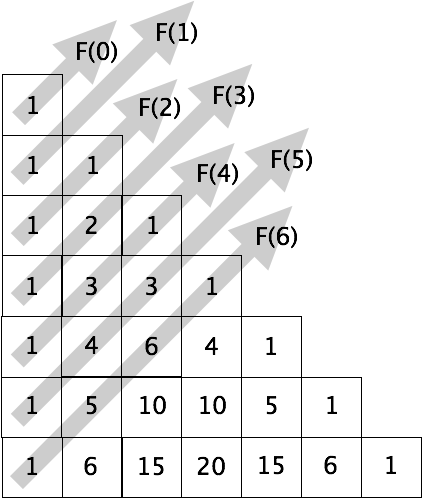
\includegraphics[scale=0.3]{FiguresMaths//FiboPascal1}
\caption{Obtaining Fibonacci numbers as the sums of diagonal elements of the left-justified Pascal Triangle.}
\label{fig:FiboPascal}
\end{center}
\end{figure}

\begin{prop}
\label{thm:FibNo+BinomCoeff}
For all $n \in \N$, the Fibonacci number $F(n)$ is the sum of the
first $\lceil (n+1)/2 \rceil$ binomial coefficients $\displaystyle {k
  \choose i}$ such that $k+i = n$.  Symbolically,
\begin{equation}
\label{eq:FibNo+BinomCoeff}
F(n) \ = \ {n \choose 0} \ + \ {{n-1} \choose 1} \ + \cdots + \ 
{{\lfloor (n+1)/2 \rfloor} \choose {\lceil (n+1)/2 \rceil -1}}.
\end{equation}
\end{prop}

\begin{figure}[htb]
\begin{center}
        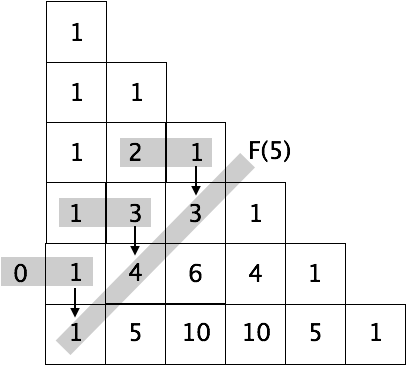
\includegraphics[scale=0.3]{FiguresMaths//FiboPascal2}
\caption{Each term of the diagonal is obtained by summing the two preceding ones.}
        \label{fig:FiboPascalExplanation}
\end{center}
\end{figure}

\begin{proof}[Sketch]
Because of the heavy calculational content of a complete proof, we
provide here just a short sketch.

Fig.~\ref{fig:FiboPascalExplanation} depicts a portion of Pascal's
Triangle with shaded diagonal and horizontal annotations.  The shaded
diagonal annotation depicts the three numbers in the Triangle that
sum to the Fibonacci number $F(5)$.
\begin{enumerate}
\item
Looking at the three horizontal shaded areas {\em individually}
illustrates how each of the three numbers on the shaded diagonal (1, 4, 3),
being a binomial coefficient, arises as a sum of two numbers on the
preceding row of the array---as instantiations of the formation rule
for Pascal's Triangle.  The illustrated instance of the rule asserts
that:
\[
\begin{array}{ccccccc}
{\displaystyle {5 \choose 0}}
 & = &
{\displaystyle 0 + {4 \choose 0} }
 & = &
0 + 1
 & = & 1 \\ \\
{\displaystyle {4 \choose 1}}
 & = &
{\displaystyle {3 \choose 0} + {3 \choose 1} }
 & = &
1 + 3
 & = & 4 \\ \\
{\displaystyle {3 \choose 2}}
 & = &
{\displaystyle {2 \choose 1} + {2 \choose 2} }
 & = &
2 + 1
 & = & 3
\end{array}
\]
\item
Looking at the three horizontal shaded areas {\em in tandem}
illustrates that the numbers along the shaded diagonal are sums of the
numbers along the two diagonals that are above the shaded one---as
instantiations of the formation rule for Fibonacci numbers.  The
illustrated instance of the rule asserts that
\[ F(5) \ = \ F(4) + F(3) \ = \ 5 + 3 \ = \ 8. \]
\end{enumerate}

The preceding reasoning provides the infrastructure of an induction
that will prove that the proposition holds for every Fibonacci
number.  As suggested by the statement of the proposition, the
required calculations on indices can obscure the rather elegant basis
for the result.
\qed
\end{proof}

%Another way to write this relation is by the following expression:
%$F_n = binomial (n,0,1 ...)$


\subsubsection{Alternative origins for the Fibonacci sequence}
\label{sec:Fibonacci-other-recurrences}

Although the classical recurrence (\ref{eq:Fibonacci-defn}) is the
structurally simplest generator of the Fibonacci sequence, there exist
other generators that are not much more complex.  We now present
several alternative ways to generate the sequence: (A) two other
multi-linear recurrences; (B) a family of binary generating
recurrences; (C) a combinatorial approach.

\paragraph{A. Two multi-linear generating recurrences}
\index{Fibonacci sequence!additional multi-linear generating recurrences}
\index{Fibonacci numbers!additional multi-linear generating recurrences}


\begin{prop}
\label{thm:FiboSum-1}
For all integers $n \geq 2$,
\begin{eqnarray}
\label{eq:multilinear-Fib-1}
F(n) & = &
1 \ + \ F(0) \ + \ F(1) \ + \ F(2) \ + \cdots + \ F(n-2) \\
\nonumber
     & = &
1 \ + \ \sum_{k=0}^{n-2} F(k)
\end{eqnarray}
\end{prop}

\begin{proof}
We proceed by induction.

\noindent
The {\em base case}, $n=2$, holds because $F(2) = 2 =  1 + F(0)$.

\noindent 
Assume, {\em for induction}, that 
(\ref{eq:multilinear-Fib-1}) holds for all arguments $2 \leq m < n$.

\noindent
We {\em extend} the induction as follows.  Our inductive hypothesis
assures us that for all $n \geq 3$,
\[ F(m-1) \ = \ 1 \ + \ F(0) \ + \ F(1) \ + \ F(2) \ + \cdots + \ F(n-3). \]
Combining this with the classical recurrence
(\ref{eq:Fibonacci-defn}), we therefore have
\begin{eqnarray*}
F(n) & = & F(n-2) \ + \ F(n-1) \\
     & = &
F(n-2) \ + \ 1 \ + \ F(0) \ + \ F(1) \ + \ F(2) \ + \cdots + \ F(n-3)
\end{eqnarray*}

\noindent
This extends the induction and completes the proof.
\qed
\end{proof}

\medskip

While recurrence (\ref{eq:multilinear-Fib-1}) in
Proposition~\ref{eq:multilinear-Fib-1} employs all of the Fibonacci
numbers up to the desired bound, recurrence
(\ref{eq:multilinear-Fib-2}) in the next proposition employs only
every other such number.

\begin{prop}
\label{thm:FiboSum-2}
For all integers $n \geq 2$,
\begin{equation}
\label{eq:multilinear-Fib-2}
F(n) \ \ = \ \
F(n-1) \ + \ F(n-3) \ + \ F(n-5) \ + \cdots + \ 1
\end{equation}
We thereby sum every other Fibonacci number as long as we can.
\end{prop}
%{\Denis Attention here on the values of C, verify! I think the
%constant are the same, see details in the next paragraph...}

\begin{proof}
We develop the claimed summation (\ref{eq:multilinear-Fib-2}) by
iteratively expanding the righthand term (i.e., $F(n-2)$) of the
classical recurrence (\ref{eq:Fibonacci-defn}).  This expansion begins
\begin{eqnarray}
\label{eq:multilinear-Fib-3}
F(n)
& = &
F(n-1) \ + \ F(n-2) \\
\nonumber
& = &
F(n-1) \ + \ F(n-3) \ + \ F(n-4) \\
\nonumber
& = &
F(n-1) \ + \ F(n-3) \ + \ F(n-5) \ + \ F(n-6)
\end{eqnarray}
Note that all term-indices in the expanded summation have the same
parity: The sequence of expanded indices begins $n-2$, $n-4$, $n-6$,
\ldots, so successive expanded indices always differ by $2$;
therefore, the index $n-k$ that we expand always has the same parity
as $n$.

We continue the expansion process of (\ref{eq:multilinear-Fib-3}) as
long as we can---i.e., until we encounter either $F(0)$, in the case
of even $n$, or $F(1)$, in the case of odd $n$.  In both cases, ``we
have run out of Fibonacci numbers'', so the expansion
terminates---coincidentally with the final term $1$.  \qed
\end{proof}

%{\Denis I found a little mistake in the original writing, redoing the calculations, t appears the constants are the same in both cases... Please, check my calculus}

\paragraph{B. A family of binary generating recurrences}
\index{Fibonacci sequence!a family of binary generating recurrences}
\index{Fibonacci numbers!a family of binary generating recurrences}

What we have earlier called ``generating recurrences'' or ``formation
rules'' for binomial coefficients and Fibonacci numbers can also be
viewed as (mathematical) identities on the quantities of interest.  In
our usage, the line between ``generating recurrences'' and
``identities'' centers on computational issues: multilinear
recurrences can feasibly be used to generate the desired numbers;
nonlinear recurrences such as we expose in this subsection will likely
not be used as generators.  Indeed, for several of the results we
cover here, it is the methodology of proof and analysis that we wish
to stress.

\begin{prop}
\label{thm:Fib-higher-indices}
For all $n \in \N$ and $0 < k < n$
\begin{equation}
\label{eq:Fib-higher-indices}
F(n) \ = \ F(k) \cdot F(n-k) \ + \ F(k-1) \cdot F(n-k-1).
\end{equation}
\end{prop}

Of course, the classical recurrence (\ref{eq:Fibonacci-defn}) is
instance $(k = 1)$ of the family of recurrent equations
(\ref{eq:Fib-higher-indices}).

\begin{proof}
We first explain how one might guess at the existence of the family of
recurrences (\ref{eq:Fib-higher-indices}), and then we validate the
recurrences in the family.

We begin with the classical recurrence (\ref{eq:Fibonacci-defn})
and iteratively use this recurrence to ``expand'' the classical
recurrence.  In detail, we begin by combining the first two instances
of (\ref{eq:Fibonacci-defn}), namely,
\[
\begin{array}{lcrrr}
F(n)   & = & F(n-1) & + & F(n-2) \\
F(n-1) & = & F(n-2) & + & F(n-3)
\end{array}
\]
and we combine them algebraically to produce the following.
\[ F(n) \ = \ 2 F(n-2) \ + \ F(n-3). \]
And then we iterate!  The following table illustrates the result of
the first four iterations of the process.
\[
\begin{array}{ccrcrcrcrcrcr}
F(n) & = & F(n) & + & F(n-1) \\
     & = &      &   & 2 F(n-1) & + & F(n-2) \\
     & = &      &   &          &   & 3 F(n-2) & + & 2 F(n-3) \\
     & = &      &   &          &   &          &   & 5 F(n-3) & + & 3 F(n-4)  \\
     & = &      &   &          &   &          &   &          & + & 8
F(n-4) & + & 5 F(n-5)  \\
 & \vdots  &  & \vdots  &  &  \vdots &  & \vdots
 &  & \vdots  &   & \vdots  & 
\end{array}
\]
Note that the coefficients of the successive occurrences of the
Fibonacci numbers $F(i)$ that occur in our table are themselves
Fibonacci numbers.  By analyzing the emerging pattern---{\em remember
  our advice in Chapter~\ref{ch:doingmath} to always look for
  patterns}---we arrive at the family (\ref{eq:Fib-higher-indices})
of recurrent equations.
\bigskip

\noindent \fbox{
\begin{minipage}{0.95\textwidth}
Keep in mind that, at this point, we are still in the realm of
  conjecture!  We must now verify the universal validity of the
  family.
\end{minipage}
}
\bigskip

We proceed by induction on the number $k$ of iterated expansions of
the classical recurrence (\ref{eq:Fibonacci-defn}).

The {\em basis for our induction} resides in the observation we shared
right after stating the proposition: Instance $(k = 1)$ of the posited
family of recurrent equations is just the classical recurrence
(\ref{eq:Fibonacci-defn}).

Let us assume that instance $k$ of family
(\ref{eq:Fib-higher-indices}), namely, the equation
\[ F(n) \ = \ F(k) \cdot F(n-k) \ + \ F(k-1) \cdot F(n-k-1) \]
is valid.  {\em Note that validity requires that $k < n-1$.}
Let us observe, under the validity assumption, the result of producing
instance $k+1$ from this instance.  We algebraically combine the
just-cited equation with the following instantiation of the classical
recurrence:
\[ F(n-k) \ = \ F(n-k-1) \ + \ F(n-k-2) \]
We find that
\begin{eqnarray*}
F(n) & = & F(k) \cdot F(n-k) \ + \ F(k-1) \cdot F(n-k-1) \\
     & = & F(k) \cdot \big[ F(n-k-1) \ + \ F(n-k-2) \big]  \ +
             \ F(k-1) \cdot F(n-k-1) \\
     & = & \big[ F(k) \ + \ F(k-1) \big] \cdot F(n-k-1) \ + \ F(k)
             \cdot F(n-k-2) \\
     & = & F(k+1) \cdot F(n-k-1) \ + \ F(k) \cdot F(n-k-2).
\end{eqnarray*}
The induction is thus extended, which establishes the proposition.
\qed 
\end{proof}


\paragraph{C. A combinatorial setting for the Fibonacci numbers}
\index{Fibonacci sequence!in binary strings with no consecutive $1$s}
\index{Fibonacci numbers!in binary strings with no consecutive $1$s}
\index{Fibonacci sequence!a combinatorial setting}
\index{Fibonacci numbers!a combinatorial setting}

In Section~\ref{sec:Fibonacci-story}, we described several settings in
which one can observe the Fibonacci sequence.  The settings we chose
arose in nature---rabbits, pineapples, etc.  We now describe a {\em
  mathematical} setting in which the sequence occurs.  In common with
our rabbits and pineapples, this setting does not involve the solution
of a system of recurrent equations.  In common with our equational
settings, this setting is purely mathematical.

Our setting is {\em combinatorial} in nature, in the sense that the
Fibonacci numbers emerge as we count instances of some phenomenon.
But, of course, the generating recurrence is still present; it is just
camouflaged by the counting.

For each positive integer $n$, let $S_n$ be the set of all length-$n$
binary strings in which {\em every occurrence of bit $1$ is directly
  preceded by an occurrence of bit $0$}.  Table~\ref{tab:comb-FIB}
provides the first few instances of $S_n$, with their cardinalities.
\begin{table}[hbt]
\label{tab:comb-FIB}
\caption{The first few instances of $S_n$, with their cardinalities.}
\[
\begin{array}{|c|c|c|}
\hline
n = & S_n =               & |S_n| = \\
\hline
0   & \{ \varepsilon\}    & 1 \\ 
1   & \{ 0 \}             & 1 \\
2   & \{ 00, 01 \}        & 2 \\
3   & \{ 000, 001, 010 \} & 3 \\
\hline
\end{array}
\]
\end{table}


\begin{prop}
\label{thm:FIBO-from-sparse-bitstrings}
For each positive integer $n$, the cardinality of the set $S_n$, which
consists of all length-$n$ binary strings in which each occurrence of
a $1$ is directly preceded by a $0$, is the Fibonacci number $F(n)$.
\end{prop}

\begin{proof}
By definition, every binary string $w \in S_n$ ends either with $0$ or
with $01$.
\begin{itemize}
\item
If $w$ ends with $0$, then it has the form $w = x0$, where the prefix
$x$ is a binary string of length $n-1$; moreover, $x$ must belong to
$S_{n-1}$ in order for $w$ to belong to $S_n$.  $S_n$ therefore
contains $|S_{n-1}|$ strings of this form.

\item
If $w$ ends with $01$, then it has the form $w = y01$, where the
prefix $y$ is a binary string of length $n-2$; moreover, $y$ must
belong to $S_{n-2}$ in order for $w$ to belong to $S_n$.  $S_n$
therefore contains $|S_{n-2}|$ strings of this form.
\end{itemize}

The preceding reasoning implies that the cardinalities of the sets
$S_n$ obey the following recurrence.
\[
\begin{array}{ccll}
|S_0| & = & 1 & \mbox{see Table~\ref{tab:comb-FIB}} \\
|S_1| & = & 1 & \mbox{see Table~\ref{tab:comb-FIB}} \\
|S_n| & = & |S_{n-1}| \ + \ |S_{n-2}| & \mbox{see preceding analysis}
\end{array}
\]
The preceding recurrence is just a relabeled version of the classical
recurrence (\ref{eq:Fibonacci-defn}).  The Proposition follows.  \qed
\end{proof}



\subsubsection{$\oplus$  A closed-form expression for the $n$th Fibonacci number}
\label{sec:Fib-Golden-Ratio}


The Fibonacci series is given by the recurrence:
$F(n+1) = F(n) + F(n-1)$.
The characteristic equation is thus given by:
$x^2 = x + 1$ or $x^2 - x - 1 = 0$ whose roots are determined by solving the equation for $a=1$ and $b=c=-1$.

$\Delta = b^2 - 4.a.c = 1+4 = 5$

As both roots are centered apart $x^*=\frac{-b}{2a}= \frac{1}{2}$, corresponding to $y^*= -\frac{\Delta}{4a} = -\frac{5}{4}$, we can rewrite the equation as:

$(x-\frac{1}{2})^2 - \frac{5}{4} = 0$

This gives: $(x-\frac{1}{2})^2 = \frac{5}{4}$ and thus, $x_1-\frac{1}{2} = - \sqrt{\frac{5}{4}}$ or $x_2-\frac{1}{2} = + \sqrt{\frac{5}{4}}$.

The last value is the Golden ratio: $\Phi = \frac{1}{2} + \sqrt{\frac{5}{4}} = \frac{1+\sqrt{5}}{2}$

\begin{figure}[htb]
\begin{center}
       \includegraphics[scale=0.3]{FiguresArithmetic/SecondDegreeFibo}
\caption{Determining graphically the Golden ratio (second root, denoted by $x_2$).}
\label{fig:SecondDegreeFibo}
\end{center}
\end{figure}

We close our survey of the Fibonacci numbers by exposing a {\it
  closed-form expression}\footnote{The term ``closed-form expression''
  is defined and illustrated in Section~\ref{sec:special-arithmetic
    sums}.A.}~for the numbers in this fascinating family.  The
detailed derivation of this form is beyond the scope of this text, so
we settle for a heuristic explanation of the closed-form expression.
By ``heuristic'', we mean here the kind of intuitive explanation that
mathematicians often use to garner intuition during the exploratory
phase of studying a complex topic. 

If you write out a sufficiently long initial sequence of Fibonacci
numbers, then you observe that they grow quite fast.  Indeed, by this
point in the text, you have hopefully ``played'' with enough sequences
that you might guess that the Fibonacci numbers grow exponentially
with the index $n$.  That is, you might guess that there exists a base
$\beta > 1$ and a constant of proportionality $c > 0$ such that $F(n)
= c \beta^n$, at least approximately.  In order to (hopefully!)~garner
intuition for the actual growth behavior of the Fibonacci numbers, let
us observe an important corollary of this guess.  If the guess were
true, then it would combine with the classical recurrence
(\ref{eq:Fibonacci-defn}) in the following way.
\[ \begin{array}{cccll}
(1) & F(n) & = & c \beta^n
      & \mbox{ by our guess} \\
(2) & F(n) & = & F(n-1) \ + \ F(n-2)
      & \mbox{ by recurrence (\ref{eq:Fibonacci-defn})}
\end{array}
\]
By combining (1) and (2), we therefore find that
\[ \beta^n \ = \ \beta^{n-1} \ + \ \beta^{n-2} \]
so that $\beta^n$ is a root of the quadratic equation
\[
x^2 - x - 1 \ = \ 0
\]
By the quadratic formula (see
Proposition~\ref{thm:quadratic-formula}), this polynomial has two roots 
$\Phi \ = \ {\displaystyle \frac{1+\sqrt{5}}{2}}$ \ \ and \ \
$\Phi' \ = \ {\displaystyle \frac{1-\sqrt{5}}{2}}$

%{\Denis well done, I like the way this is presented, but where is the  section on quadratic formula?}
%{\Arny Proposition~\ref{thm:quadratic-formula}) is in Chap 5; this is in Chap 8}


\noindent
Note that $\Phi$, which is known as the \textit{golden ratio},
\index{golden ratio} exceeds $1$ while $\Phi'$ does not.  Since we
know that the Fibonacci numbers {\em grow} with $n$ rather than shrink
with $n$, our initial guess would assign $F(n)$ the value
\[
F(n) \ = \ \Phi^n \ = \ {\displaystyle \left( \frac{1+\sqrt{5}}{2} \right)^n }
\]
In fact, this guessed value of $F(n)$ is off by only a small constant
factor, at least for very large values of $n$, in the sense of part
(a) of the following result.  Part (b) of the result actually provides
a closed-form expression for $F(n)$.
\index{Fibonacci numbers!closed-form expression}

\begin{prop}
\label{thm:FibNo-GoldenRatio}
{\bf (a)} {\rm (An approximating expression)}
For all sufficiently large $n$,
\[ F(n) \ \approx \
\frac{1}{\sqrt{5}} \left(\frac{1+\sqrt{5}}{2} \right)^n
\]
The meaning of the symbol ``$\approx$'' here means that the error
incurred by approximating $F(n)$ via this expression shrinks
exponentially as $n$ grows.

\medskip

\noindent{\bf (b)} {\rm (An exact expression)}
For all $n$,
\[ F(n) \ = \ 
\frac{1}{\sqrt{5}} \left( \left(\frac{1+\sqrt{5}}{2} \right)^n -
\left(\frac{1-\sqrt{5}}{2} \right)^n \right)
\]
\end{prop}


%%%%%%%%%%%%%%%%%%%%%%%%%%%%%%%%%%%%%%%


\section{$\oplus$ Recurrences ``in action'': The Token Game}
\label{sec:TokenGame}

In order to truly appreciate the power of recurrences as an analysis
tool, one must witness them ``in action''.  To this end, we now
describe the (single-player) combinatorial {\it Token Game}.  By
employing recurrences to analyze plays of the game, we are able to
derive an optimal strategy for playing the game.

\subsection{Rules of the Game}
\label{sec:TokenGame-Rules}

\noindent {\it The equipment}.
For each $n \in \N^+$, the order-$n$ version of the Token Game is
played with a {\it bank} which has $n$ slots, labeled $1$, \ldots,
$n$, and with a {\it pile} of $n$ tokens.

\medskip

\noindent {\it Initial and terminal configurations}.
Each play of the game begins with the bank empty and the pile full, as
depicted in Fig.~\ref{fig:jeujetonsInit}.
\begin{figure}[htb]
\begin{center}
        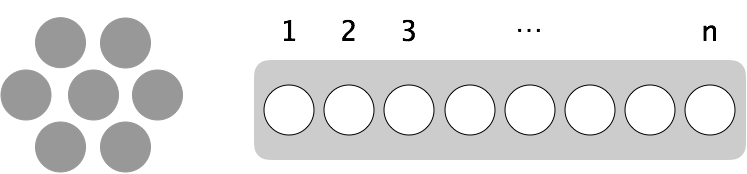
\includegraphics[scale=0.35]{FiguresMaths/GameTokenInit.png}
\caption{The initial configuration of the Token Game: Each of the $n$
  tokens appears as a grey circle, and the empty bank has $n$ slots.
  In the figure, $n=8$.}
        \label{fig:jeujetonsInit}
\end{center}
\end{figure}
The goal of each play is to transfer all $n$ tokens from the pile into
the bank.

\medskip

\noindent {\it The repertoire of Game moves}.
The player transfers tokens from the pile to the bank by executing a
sequence of {\it moves}.  Each successive move has one of the
following types.
\begin{enumerate}
\item
Change the state of bank-slot \#$1$, which is the first (i.e.,
leftmost) slot in the bank:

If slot \#$1$ is empty, then move a token from the pile to that slot.

If slot \#$1$ is full (i.e., contains a token), then remove this token
and return it to the pile; see Fig.~\ref{fig:rule1}.
\begin{figure}[h]
\begin{center}
        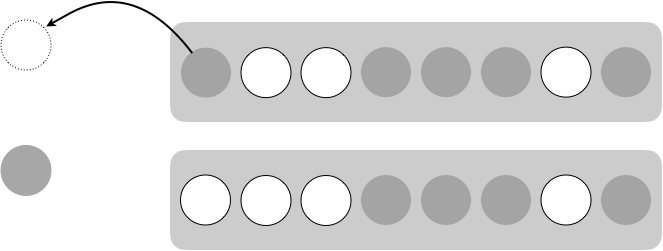
\includegraphics[scale=0.3]{FiguresMaths/GameTokenRule1.png}
\caption{(TOP) Slot \#1 contains a token.  (BOTTOM) Therefore, remove
  it (i.e., move it back to the pile).}
        \label{fig:rule1}
\end{center}
\end{figure}

\item
Change the state of the bank-slot---call it slot \#$s$---that is
immediately to the right of the first (i.e., leftmost) {\em empty}
slot:

If slot \#$s$ is empty, then move a token from the pile to that slot.

If slot \#$s$ is full (i.e., contains a token), then remove this token
and return it to the pile; see Fig.~\ref{fig:rule2}.
\begin{figure}[htb]
\begin{center}
        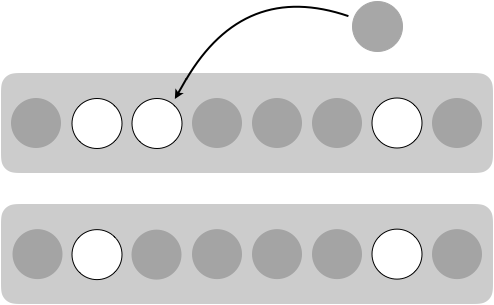
\includegraphics[scale=0.3]{FiguresMaths/GameTokenRule2.png}
\caption{(TOP) Bank-slot \#$s$, which is immediately to the right of
  the first empty slot ($s=3$ in this example) is empty.  (BOTTOM)
  Therefore, move a token from the pile into slot \#$3$.}
        \label{fig:rule2}
\end{center}
\end{figure}
\end{enumerate}

\medskip

\noindent {\it Objective of a play of the Game:} To minimize the
number of moves from an initially empty bank to the finally full bank.


%Note that Rule 1 refers only to the slot whose full/empty status can
%change in this step, whereas Rule 2 depends on the status of slots
%whose full/empty status cannot change in this step.

\subsection{An Optimal Strategy for Playing the Game}
\label{sec:Token-Game-Strategies}

The question is how the player should choose successive moves, 
with the goal of filling the bank as quickly as possible. 
While one can garner some strategic observations about how to play the
Game by looking at small instances.
The basic case $n=1$ is simply to fill the slot by a Type-$1$ move.
For $n=2$, we must first play a Type-$2$ move followed by a Type-$1$ move. 
An observation of playing the Game for the next small values of $n$ (say $n=3, 4$ or $5$)
evidences that the initial move involves alternatively both types: a Type-$1$ move if $n$ is odd
and a Type-$2$ move if it is even. 
Another easy observation is: Do not play
two successive moves of the same type, because the second one just undoes the first.
Thus, as the moves are imposed, a strategy is easy to deduce: 
start by the right initial move depending of the parity of $n$ and change alternatively the type
of the successive moves.
How are we sure that the game provides the required terminal state? How to evaluate its cost?

The answer is given by specifying a {\em recursive} solution to
the game, which can be proved optimal using recurrences.

\ignore{
While one can garner some strategic observations about how to play the
Game by playing small instances---a trivial example: 


%WhileEven is not easy to describe and its cost is not easy to
%establish.  We lay the groundwork for devising an optimal strategy
%for playing the game by making some observations.  The analysis of
%the game for some particular values of $n$ leads to some evidences
%(looking at the first ranks): First, in the even case, the process
%should start by putting the second token while in the odd case, we
%should start to fill the first position.  Then, the first token is
%flipped every double steps, the second one every four steps and so
%on.  Second observation: both rules are applied alternatively (this
%is obvious for Rule 1 since applying it twice consecutively leads to
%the initial position, and easy to check for Rule 2 on the first
%ranks).
}

\bigskip

A recursive solution for Game instances with $n > 2$ can be derived
from the following reasoning.

A token can be placed into the last bank-slot via the type-$2$ move
\begin{center}
{\sc move token from pile into bank-slot} $n$.
\end{center}
In order for this move to be eligible for execution, the bank must be
in the following configuration, reading rightward from bank-slot $1$:
\[ \big[ \mbox{tokens in slots } \ 1, 2, \ldots, n-2 \big],
 \big[ \mbox{no token in slot } \ n-1 \big],
 \big[ \mbox{no token in slot } \ n \big]
\]
This requires that the first $n-2$ slots have been filled.
Notice here that this number has the same parity as $n$.
Once  having achieved this configuration, and then executed the move
\begin{center}
{\sc move token from pile into bank-slot} $n$,
\end{center}
\ignore{the player can execute a sequence of $n-2$ type-$2$ moves of the form
\begin{center}
{\sc move token from bank-slot} \ $k$ \ {\sc to the pile},
\end{center}
for $k = n-2, \ n-3, \ldots, \ 1$, in turn.  
}
At this point, if one
henceforth ignores the token in bank-slot $n$, then the player is now
confronted with the initial configuration of the order-$(n-1)$ version
of the Game.  You can see the recursion coming!

Thus, the Game can be played via a recursion that iteratively executes
the ``super-steps'' depicted in Figure~\ref{fig:jeujetonsPrinciple},
on successively smaller banks and piles.
\begin{figure}[htb]
\begin{center}
        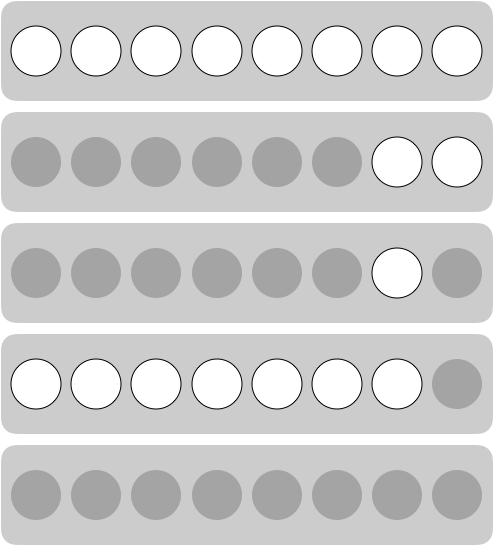
\includegraphics[scale=0.3]{FiguresMaths/GameTokenPrinciple.png}
\caption{A schematic of the recursive play of the current-sized
  version of the Game.  The top four bank configurations indicate the
  iterating four supersteps in the recursions.  The bottom bank
  configuration is the final one: the bank is entirely filled. }
        \label{fig:jeujetonsPrinciple}
\end{center}
\end{figure}

Let summarize these super-steps:
\begin{enumerate}
\item
{\it Topmost bank configuration $\longrightarrow$ Second bank
  configuration}

Move tokens into the leftmost $n-2$ slots of the bank, leaving the
rightmost two slots empty.

\item
{\it Second bank configuration $\longrightarrow$ Third bank configuration}

Move a token into bank-slot $n$, i.e., the current rightmost slot

\item
{\it Third bank configuration $\longrightarrow$ Fourth bank configuration}

Empty  bank-slots $1, 2, \ldots n-1$; i.e., leave the current
rightmost slot filled, but empty all slots to its left.

\item
{\it Final bank configuration}

The Game is complete!
\end{enumerate}

%Thus, flipping the first tokens of the same color is different if they are all blue or red.
%Notice that flipping the first reds can be obtained using the reverse process as for the blue ones (see coding at the end of this document).

\ignore{\medskip

We can specify the preceding recursive algorithm in the following more
formal format:

\medskip

\begin{tabular}{|l|c|ll|}
\multicolumn{4}{l}{{\bf Recursive-Procedure} Fill-Bank($n$)} \\
\hline
\multicolumn{4}{l}{/* Fill the leftmost $n$ slots of the currently
  empty bank */} \\
\hline
\hline
\underline{\bf Case} & \underline{\bf Move-sequence} & 
\multicolumn{2}{c}{\underline{\bf Action}} \\ 
$n=1$ &   & Move-Token to slot \#$1$ & via a Type-$1$ move \\
\hline
$n=2$ & 1 & Move-Token to slot \#$2$ & via a Type-$2$ move \\
      & 2 & Move-Token to slot \#$1$ & via a Type-$1$ move \\
%PutToken(2) -- Rule 2 -- and then PutToken(1) -- Rule 1
\hline
$n>2$ & 1 & Fill-Bank($n-2$) & via recursive invocation \\
%\item fillBank(n-2)
      & 2 & via a Type-$2$ move \\
%\item PutToken(n)
      & 3 & Erase leftmost $n-2$ bank-slots & as described in text \\
%\item EmptyBank(n-2)
      & 4 & Fill-Bank($n-1$) & via recursive invocation \\
%\item FillBank(n-1)
\hline
\end{tabular}
}


\subsection{An analysis of the recursive strategy}
\label{sec:analysis-of-Token-Game}

We now develop an analysis of our recursive strategy for playing the
Token Game.  Not surprisingly, the analysis is embodied in a {\it
  recurrence} for the cost of playing the Game as a function of the
bank-size $n$.  Also not surprisingly, the structure of the recurrence
mirrors the recursion structure of our playing strategy.

For $i = 1, \ldots, n$ let $F(i)$ denote the cost for filling the
bank-slots from slot \#$1$ through slot \#$i$, measured in terms of
the number of atomic moves, each of the form {\sc place a token} or
{\sc remove a token}.  Because of the dual forms of our atomic
moves---each move fills one slot that is empty or empties one slot
that is full---the cost of filling an empty length-$i$ prefix of the
bank with tokens equals the cost of emptying a full length-$i$ prefix
of the bank.  The total cost of a play of the Game is, by definition,
the cost of filling the initially empty $n$-slot bank with tokens.

\begin{prop}
\label{thm:f-cost of TokenGame}
Let $F(n)$ be the cost of a play of the $n$ bank-slot version of the
Token Game.  For all $n \in \N^+$, the value of $F(n)$ is
\begin{equation}
\label{eq:f-cost:Token-Game}
F(n) \ = \ \left\{
\begin{array}{ll}
 \frac{1}{3} \left( 2^{n+1} -1 \right)
  & \mbox{  if $n$ is odd} \\
 \frac{1}{3} \left( 2^{n+1} -2 \right)
  & \mbox{  if $n$ is even}
\end{array}
\right.
\end{equation}
\end{prop}

\begin{proof}
Our discussion has revealed that the analysis of our recursive playing
strategy resides in solving the following recurrence.
\begin{equation}
\label{eq:Token-cost-recurrence}
F(n) \ = \ \left\{
\begin{array}{ll}
1 & \mbox{ if } \ n=1 \\
2 & \mbox{ if } \ n=2 \\
% F(n-2) + 1 + F(n-2) + F(n-1) = 
F(n-1) \ + \ 2 F(n-2) + 1 & \mbox{ if } \  n > 2
\end{array}
\right.
\end{equation}
\medskip

\noindent \fbox{
\begin{minipage}{0.95\textwidth}
There is a point to clarify here since the moves of the Game are not \textit{symmetric}
(we proceed from left to right). 

The recursive solution involves a step to empty a bank of size $n-2$.
It appears that filling or emptying a bank are mirroring operations. 
We let the reader check on small instances of $n$ that the operations for emptying 
the bank are the reverse operations of filling the bank (the first step becomes the last one,
the second one becomes the penultimate and so on).

This observation can be proved formally as follows.

Let $F^{-1}$ denote the emptying operation. 
The cost expression of the recursive solution is precisely:

\begin{equation}
F(n) \ = \ \left\{
\begin{array}{ll}
1 & \mbox{ if } \ n=1 \\
2 & \mbox{ if } \ n=2 \\
% F(n-2) + 1 + F(n-2) + F(n-1) = 
F(n-2) \ + 1 \ + F^{-1}(n-2) \ + F(n-1) & \mbox{ if } \  n > 2
\end{array}
\right.
\end{equation}

It is not difficult to derive a recursive solution for the emptying operation
(think that they are mirrors):
\begin{equation}
F^{-1}(n) \ = \ \left\{
\begin{array}{ll}
1 & \mbox{ if } \ n=1 \\
2 & \mbox{ if } \ n=2 \\
F^{-1}(n-1) \ + F(n-2)  \ + 1 \ + F^{-1}(n-2) & \mbox{ if } \  n > 2
\end{array}
\right.
\end{equation}

Now, make the difference between both expression:

$F(n) - F^{-1}(n)$

$= F(n-2) \ + 1 \ + F^{-1}(n-2) \ + F(n-1) $

$- F^{-1}(n-1) \ - F(n-2)  \  1 \ - F^{-1}(n-2)$

$= F(n-1) - F^{-1}(n-1) = \cdots = F(1) - F^{-1}(1) = 0$

Thus, the cost of $F(n)$ and $F^{-1}(n)$ are the same!
\end{minipage}
}
\bigskip

We can dramatically simplify recurrence
(\ref{eq:Token-cost-recurrence}) by focusing on the function
\[ g(n) \ \eqdef \ F(n) \ + \ F(n-1) \ \ \mbox{ for } \ n \geq 2 \]
instead of on $F$.  Elementary calculation based on
(\ref{eq:Token-cost-recurrence}) shows that $g(n)$ satisfies the
recurrence
\begin{equation}
\label{eq:g-Token-cost-recurrence}
g(n) \ = \ \left\{
\begin{array}{ll}
3 & \mbox{ if } \ n=2 \\
2 g(n-1) + 1 & \mbox{ if } \  n > 2
\end{array}
\right.
\end{equation}
We have, thereby, replaced the {\em bilinear} recurrence
(\ref{eq:Token-cost-recurrence}) by the {\em (singly) linear}
recurrence (\ref{eq:g-Token-cost-recurrence}).  We learned in
Section~\ref{sec:geometric-sums}---specifically, see
Proposition~\ref{thm:sum-finite-geometric-series}---how to evaluate
the geometric summations that solve recurrences such as
(\ref{eq:g-Token-cost-recurrence}).  In our case, we find that
%If we add $F(n-1)$ in both sides of the previous expression, we obtain
%a simpler equation (call $s(n)$ the sum $F(n)+F(n-1)$ $n \geq 2$, in
%particular, $s(2) = 2+1$):
%
%$F(n) + F(n-1) = 2.F(n-1) + 2.F(n-2) +1$
%$s(n) = 2.s(n-1)+1 = 2.(2.s(n-2)+1) + 1 = 2^2 s(n-2) + 2+ 1 = 2^3
%s(n-3) + 2^2 + 2 + 1 = ... = 2^{n-2} s(2) + 2^{n-3} + ... + 2^2 + 2 +
%1$ where $s(2) = 2+1$
\begin{equation}
\label{eq:VALUE-g-Token-cost}
g(n) \ \ = \ \ 2^{n-1} \ + \ 2^{n-2} \ + \cdots + \ 2^2 \ + \ 2 \ +
\ 1 \ \ = \ \ 2^{n} -1
\end{equation}
%
%Summing up this geometric series leads to
%$s(n) = 2^{n} -1$

\medskip

We can now return to evaluating $F(n)$ via recurrence
(\ref{eq:Token-cost-recurrence}), in the light of our analysis of
$g(n)$ in (\ref{eq:g-Token-cost-recurrence}) and
(\ref{eq:VALUE-g-Token-cost}).  We find that 
\begin{equation}
\label{eq:f-Token-cost-recurrence}
F(n) \ = \ \left\{
\begin{array}{ll}
1 & \mbox{ if } \ n=1 \\
g(n) - F(n-1) \ \ = \ \
\left(2^{n} -1\right) - F(n-1) & \mbox{ if } \ n>1
\end{array}
\right.
\end{equation}
We begin to solve the {\em singly} linear recurrence
(\ref{eq:f-Token-cost-recurrence}) for $F(n)$ using the strategy we
developed in Section~\ref{sec:geometric-sums}; namely, we expand the
recurrence in order to discern its pattern and then aanalyze the
summation that the pattern leads us to.  In this case, we find that
\begin{eqnarray*}
F(n) & = & 2^{n} - 2^{n-1} + F(n-2) + 1 -1 \\
     & = & 2^{n} - 2^{n-1} + 2^{n-2} - F(n-3) -1 \\
     & = & 2^{n} - 2^{n-1} + 2^{n-2} - 2^{n-3} + F(n-4) +1-1 \\
     &   & \vdots
\end{eqnarray*}
What we observe emerging---an inviting induction for the reader lurks
in those words---is a geometric summation of powers of $2$, with
adjacent terms {\em alternating} in sign; the terminal units, $\pm 1$,
cancel after each pair of steps.  We must be careful, though, because
the numbers of terms in the summations differ based on the parity of
$n$: when $n$ is even, the last term is $-2$; when $n$ is odd, the
last term is $-1$.

We have now reached the {\em penultimate} step in finding the value of
$F(n)$; specifically, we have derived the following parity-specified
summations.
\begin{eqnarray}
\label{eq:EVEN-f-sum}
\mbox{For even values of } \ n \ \ \
F(n) & = &
\sum_{k=1}^n \ (-1)^{k} \ 2^{k} \\
\label{eq:ODD-f-sum}
\mbox{For odd values of } \ n \ \ \ \
F(n) & = &
\sum_{k=0}^n \ (-1)^{k+1} \ 2^{k}
\end{eqnarray}
Solving these parity-specific summations for $F(n)$ requires a
moderate bit of mathematical dexterity.  For pedagogical reasons, we
illustrate two quite distinct approaches for determining the value of
$F(n)$ for the case of odd $n$: we want to expose the reader to the
quite-different intuitions that each approach elicits.  We shall then
derive the value of $F(n)$ for the case of even $n$ from the value for
the case of odd $n$.

\medskip

\noindent {\it An algebraic approach for the case of odd $n$}.
We look in detail at summation (\ref{eq:ODD-f-sum}), which specifies
$F(n)$ when $n$ is odd, and we invoke algebraic manipulation to
determine the value of $F(n)$ in this case.

In the following chain of equalities, we: gather the positive and
negative terms in summation (\ref{eq:ODD-f-sum}) [line 1 in the
  chain], perform some elementary manipulations on the result [lines 2
  and 3 in the chain], and then invoke
Proposition~\ref{thm:sum-finite-geometric-series} [line 4 in the
  chain, which evaluates the resulting geometric summation].  We
thereby find that, for odd values of $n$:
\begin{eqnarray*}
\label{eq:ODD-soln-f-sum}
F(n)
  & = &
\left(2^{n} \ + \ 2^{n-2} \ + \cdots + \ 2 \right) \ - \
  \left(2^{n-1} \ + \ 2^{n-3} \ + \cdots + \ 1 \right) \\
%    & = &
%2 \cdot \left(2^{n-1} \ + \ 2^{n-3} \ + \cdots + \ 1 \right) \ - \
%  \left(2^{n-1} \ + \ 2^{n-3} \ + \cdots + \ 1 \right) \\
    & = &
2^{n-1} \ + \ 2^{n-3} \ + \cdots + \ 1  \\
    & = &
2^{n-1} \cdot \left( 1 \ + \ \frac{1}{4} \ + \ \frac{1}{16}  \ +
\cdots + \ \frac{1}{2^{n-1}} \right) \\
    & = &
\frac{1}{3} \left(2^{n+1} - 1 \right) 
\end{eqnarray*}

\bigskip

\noindent {\it A geometric approach for the case of odd $n$}.
We begin again by looking again at summation (\ref{eq:ODD-f-sum}).
Then, noting that $2^{n-1}$ is a perfect square whenever $n$ is odd,
we set out to represent $F(n)$ as the aggregated area of a shrinking
sequence of squares, of successive dimensions
\[ 2^{(n-1)/2} \times 2^{(n-1)/2}, \ \ 2^{(n-3)/2} \times 2^{(n-3)/2},
\ \ 2^{(n-5)/2} \times 2^{(n-5)/2}, \
\ldots, \ \  1 \times 1
\]
Fig.~\ref{fig:alternatePowers2odd} depicts such a representation of
$F(7) = 64+16+4+1 = 85$.
\begin{figure} [htb]
\begin{center}
        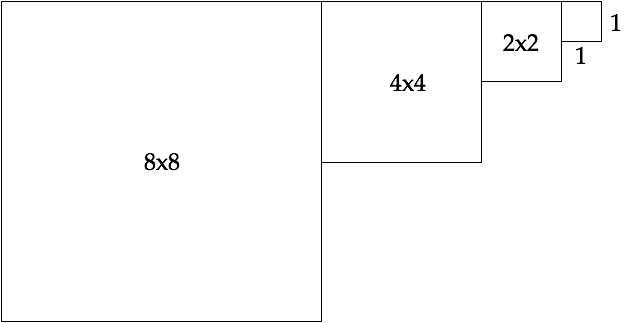
\includegraphics[scale=0.35]{FiguresMaths/alternatePowers2initOdd.png}
\caption{A representation of summation (\ref{eq:ODD-f-sum}) for the case $n=7$.}
        \label{fig:alternatePowers2odd}
\end{center}
\end{figure}
To facilitate our upcoming manipulation of the configuration depicted
in the figure, let us refer to the configuration as {\it the cascade
  of squares determined by $F(n)$}.  Note that, because each cascade
is associated with an odd value of $n$, the smallest square in the
cascade (at the far right in the figure) is the unit square, of
dimensions $1 \times 1$; hence, it contributes $+1$ to the aggregate
area of the cascade.

We can now use a geometric construction to evaluate $F(n)$ on an
arbitrary odd argument $n$.  We take three copies of the cascade in
Fig.~\ref{fig:alternatePowers2odd} and we manipulate the copies into
the form is depicted in Fig.~\ref{fig:alternatePowers2finalOdd}.  
\begin{figure} [htb]
\begin{center}
        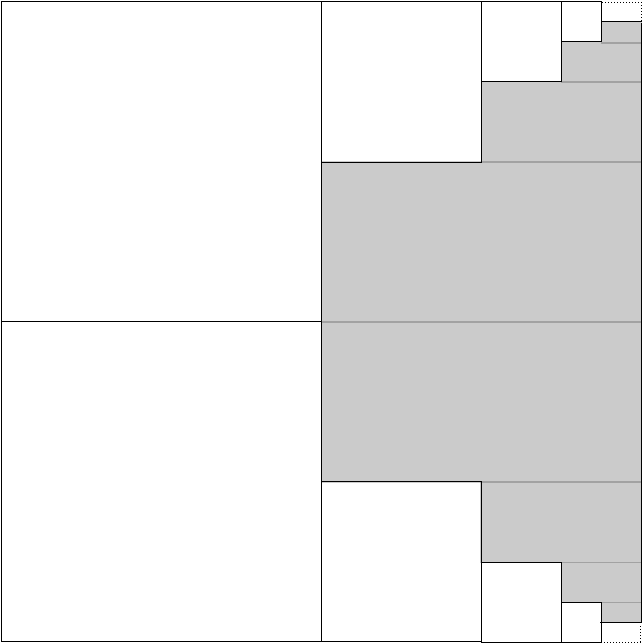
\includegraphics[scale=0.3]{FiguresMaths/alternatePowers2odd.png}
\caption{Evaluating $F(n)$ for odd $n$ by ``almost'' filling a large square.}
        \label{fig:alternatePowers2finalOdd}
\end{center}
\end{figure}
In detail:
\begin{enumerate}
\item
We choose one of the three copies as the ``anchor'' of the
construction.  We position it in space so that it serves as the upper
white cascade in Fig.~\ref{fig:alternatePowers2finalOdd}.
\item
We then take a second copy, flip it across the horizontal axis, and
abut the top edge of its largest square with the bottom edge of the
largest square in the anchor cascade.  It then becomes the lower white
cascade in Fig.~\ref{fig:alternatePowers2finalOdd}.

Note that, importantly, the abutted white cascades fit into a
$2^{(n+1)/2} \times 2^{(n+1)/2}$ square.
\begin{quote}
  {\em All of our observations about figures fitting within other
  figures are verified by direct calculations.  These calculations are
  not too hard because all squares have side-dimensions that are
  powers of $2$.}
\end{quote}
Indeed, the top edge of the top white cascade and the bottom edge of
the bottom white cascade lie, respectively, along the top and bottom
edges of the $2^{(n+1)/2} \times 2^{(n+1)/2}$ square.  {\em But}, the
cascades' edges are $1$ unit shorter that the edges of the big square;
i.e., they both have length
\[
2^{(n-1)/2} \ + \ 2^{(n-3)/2} \ + \ 2^{(n-5)/2} \ + \cdots + \ 1
\ = \ 2^{(n+1)/2} \ - 1
\]

\item
Finally, we take the third copy, color it grey, and nest it into the
abutting white cascades in the following way.
  \begin{enumerate}
  \item
Take the biggest square in the grey cascade and nest it against the
abutted biggest squares in the paired white cascades, in the manner
depicted in Fig.~\ref{fig:alternatePowers2finalOdd}.  Note that the
nest places one half of its biggest grey square abutting the biggest
white square of the top white cascade and one half abutting the
biggest white square of the bottom white cascade.  Observe (from
Fig.~\ref{fig:alternatePowers2finalOdd}) that the resulting
configuration fits within the $2^{(n+1)/2} \times 2^{(n+1)/2}$ square,
and that the fit is {\em exact} along the left and right edges, which
are shared by the abutting white cascades and the big square.

  \item
For all of the other grey square, in decreasing order of size: We
bisect---i.e., cut exactly in half---each square along its its
equator, and we nest the resulting two halves of that square
symmetrically within the abutting white cascades, in the manner
depicted in Fig.~\ref{fig:alternatePowers2finalOdd}.  Once again, we
observe that the resulting configuration fits within the $2^{(n+1)/2}
\times 2^{(n+1)/2}$ square, and that the fit is {\em exact} along the
left and right edges, which are shared by the abutting white cascades
and the big square.

The placement of the bisected squares from the grey cascade leaves two
small {\em empty} regions within the $2^{(n+1)/2} \times 2^{(n+1)/2}$
square.  The empty regions each has area $1/2$, because they are
created by the ``inadequate'' placement of the bisected unit-side
square from the grey cascade; the empty regions appear at the top
right and bottom right corners of the $2^{(n+1)/2} \times 2^{(n+1)/2}$
square.
  \end{enumerate}
\end{enumerate}

Once we have completed the described construction of the composite
object depicted in Fig.~\ref{fig:alternatePowers2finalOdd}, we
calculate that the combined areas of the three cascades is one unit
less that the area of the $2^{(n+1)/2} \times 2^{(n+1)/2}$ square
(which, of course, has area $2^{n+1}$).  We have thus shown
geometrically that $3 F(n)+1 \ = \ 2^{n+1}$, which {\em of
  course!}~agrees with the value derived algebraically in
(\ref{eq:ODD-soln-f-sum}).

\bigskip

We derive immediately the expression for even $n$ using the definition of $g(n)$:

$F(n) = 2^n -1 + F(n-1)$ for $n \geq 2$

$= 2^n -1 + \frac{1}{3} \left(2^{n} - 1 \right) $

$= \frac{1}{3} \left(2^{n+1} - 2 \right)$
\qed
\end{proof}


%
%Figures~\ref{fig:alternatePowers2even} and~\ref{fig:alternatePowers2finalEven} illustrate the construction in the even case.
%The details are left to the readers. 
%We obtain $3.F(n)+2= 2^{n+1}$ by a similar analysis.
%However, we can deduce directly the even case from the odd case by remarking that $F(2k)=2.F(2k-1) +1$.
%
%This is obtained by the basic relations $F(n) = 2^{n} - F(n-1) -1$ and $F(2k-1) = \frac{1}{3} (2^{2k} -1)$.
%
%$n=2k$, $F(n) = 2^{2k} - \frac{1}{3} (2^{2k} -1) -1 = \frac{1}{3} (2^{n+1} -2)$.
%
%\begin{figure} [h]
%\begin{center}
%        \includegraphics[scale=0.4]{FIGmaths/alternatePowers2initEven.png}
%        \caption{Representation of the alternate series of powers of $2$ for $n=6$.
%        F(6)=32+8+2.}
%        \label{fig:alternatePowers2even}
%\end{center}
%\end{figure}
%
%
%\begin{figure} [h]
%\begin{center}
%        \includegraphics[scale=0.4]{FIGmaths/alternatePowers2even.png}
%        \caption{Case odd: Geometric proof in the odd case. Notice here that there are 2 small rectangles left at the extreme corners on the right,
%        whose surface is $1$ each.}
%        \label{fig:alternatePowers2finalEven}
%\end{center}
%\end{figure}

\ignore{************
{\Arny My instinct is that the following example is not ``pretty'' or
  ``dramatic'' in the way that
  Proposition~\ref{thm:FiboSumConsecutive} is ... and it does not seem
  to teach any really new lessons.}

************
\subsubsection{Another property dealing with squares}

We will show the following property by two different methods

\noindent \textbf{Property.} 
\label{prop:FiboEmbedded}
$F(n+2)^2 = 4.F(n).F(n+1) + F(n-1)^2$ for $n \geq 2$.


The geometrical proof is obtained as depicted in Fig.~\ref{fig:fibosquareembedded} for computing $F_{n+2}^2$.

\begin{figure}[htb]
\begin{center}
        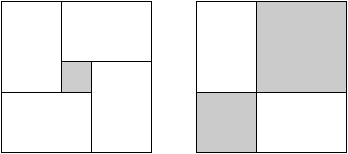
\includegraphics[scale=0.5]{FiguresMaths//FiboSquares}
        \caption{Geometric interpretation for computing $F_{n+2}^2$.}
        \label{fig:fibosquareembedded}
\end{center}
\end{figure}

Let remark that this figure might be adapted to show several properties using various decompositions of the squares and rectangles.

Another proof uses directly the definition of the Fibonacci numbers:

%$F_{n+1} + F_{n}$

$F(n+2)^2 = (F(n+1) + F(n))^2 $

$= F(n+1)^2+2.F(n+1).F(n)+F_{n}^2$

$= 4.F(n+1).F(n) - 2.F(n+1).F(n) + F(n+1)^2 + F(n)^2$

$= 4.F(n+1).F(n) + (F(n+1) - F(n))^2$

Again, using the definition of $F(n+1)$ into the square, we get the expected result:

$F(n+2)^2 = 4.F(n+1).F(n) + F(n-1)^2$
***********}

\ignore{********
{\Arny This is another one we should discuss.  As with the section
  ``Another Identity'', Cassini's Identity does not strike me as
  ``pretty'' as the ``Consecutive products'', and the proof does not
  open the way to much new methodology.  I am troubled by Carroll's
  Puzzle because its resolution builds on principles that we do not
  cover anywhere.  Since this is not a true paradox, this material
  does not belong in that section.}

{\Denis Right, put this as an exercice. }

{\Arny Both of my preceding comments build on the question, Why should
  we include this material?  Obviously, when new techniques are
  involved, or when new, highly applicable, concepts are revealed,
  then the material should be included.  In other situations, I am
  just pulled by my gut feeling.  Should we discuss?}
**************}


\ignore{**************
\subsection{$\oplus$ Cassini's Identity}
\label{sec:Cassini}
\index{Fibonacci numbers!Cassini's Identity}


\noindent \textbf{Property. (Cassini's identity)} 
\label{prop:cassini}
$F(n-1).F(n+1) = F(n)^2 + (-1)^{n+1}$ for $n \geq 1$.


The proof by induction is as follows:

\begin{itemize}
\item 
The \textbf{basis case} is straightforward since $F(0).F(2) = 2$ and $F(1)^2 +1 = 2$.

\item
The \textbf{induction step} is proved assuming the Cassini's identity holds at rank $n$.

Apply the definition of $F(n+2)$:
 
$F(n).F(n+2) = F(n) (F(n+1)+F(n)) = F(n)^2 + F(n).F(n+1)$

Replace the last term using the recurrence hypothesis:

$F(n)^2 = F(n-1).F(n+1) - (-1)^{n+1} =F(n-1).F(n+1) + (-1)^{n+2} $

Thus,
$F(n).F(n+2) = F(n).F(n+1) + F(n-1).F(n+1) + (-1)^{n+2} = F(n+1) (F(n) + F(n-1)) + (-1)^{n+2}$ 

Apply again the definition of Fibonacci sequence $F(n) + F(n-1) = F(n+1)$, we obtain:

$F(n).F(n+2) = F(n+1)^2 + (-1)^{n+2}$
\end{itemize}


The previous result (Cassini's identity) can be used for a geometrical paradox (one of the favorite puzzle of Lewis Carroll).
Consider a chess board and cut it into 4 pieces as shown in figure~\ref{paradox}, then reassemble them into a rectangle.
%Interpret this paradox.
%
\begin{figure}[htb]
\begin{center}
\label{paradox}
       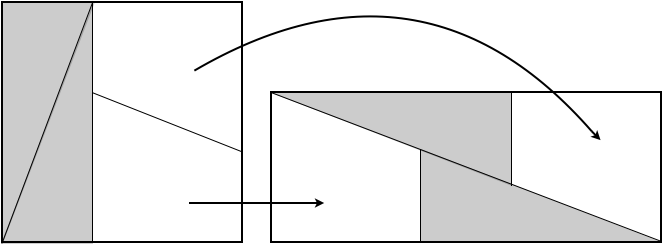
\includegraphics[scale=0.4]{FiguresMaths//FiboParadox.png}
              \caption{Construction of the rectangle after splitting the $8 \times 8$ square
              in two right $8$ by $3$ triangles and two polytopes.}
        \label{fig:FiboParadox}
\end{center}
\end{figure}

The surface of the square is $F(n)^2$ while the rectangle is $F(n+1).F(n-1)$.
In Fig.~\ref{fig:FiboParadox}, the Cassini identity is applied for $n=5$, $F(5)=8$. 
On one side, we obtain a surface of $8 \times 8 = 64$, but $13 \times 5 = 65$ on the other side!
What's wrong?

The paradox comes from the wrong representation of the diagonal of the rectangle which does not coincide with the hypothenuse
of the right triangles of sides $F(n+1)$ and $F(n-1)$.
In other words, it always remains (for any $n$) an empty space (corresponding to the unit size of the basic square of the chess board).
The greater $n$, the better the paradox because the deformation of the surface of this basic square becomes more tiny. 
***********************}

\newpage

\section{Exercices: more on recurrences}

\subsection{Karatsuba (application of the Master Theorem)} 

\noindent \textit{The aim:}
The purpose here is to put the Master theorem (section~\ref{sec:linear-recurrence-general}) in action on a classical example.

Let us first recall the generic divide-and-conquer for designing algorithms.
\bigskip

\noindent \fbox{
\begin{minipage}{0.95\textwidth}
{\it Divide and conquer} is a paradigm for designing efficient algorithms for solving problems that can be
decomposed into sub-problems.

Let consider a problem of size $n$ that can be decomposed into $p$ sub-problems.
(notice, all sub-problems have the same size n/q).
\bigskip

\noindent {\bf Principle:}
\begin{enumerate}
\item Decompose the problem into $a$ sub-problems of size $\frac{n}{q}$.
\item Solve those sub-problems.
\item Reconstruct the solution of the initial problem.
\end{enumerate}

In general, the sub-problems are solved recursively (at least until a certain threshold).
The cost is governed by the following expression:

$T(n) = p.T(\frac{n}{q}) + c_1(n) + c_3(n)$ 

where $c_1(n)$ et $c_3(n)$ are the costs of phases (1) et (3).

\end{minipage}
}
\bigskip

\noindent \textit{The problem:}
Let $A=(a_na_{n-1}\ldots a_1)_2$ and $B=(b_nb_{n-1}\ldots b_1)_2$
be two long integers, and assume $n=2^k$ for some positive integer $k$.
The goal is to compute the product $A \times B$.
\medskip

\noindent \textit{The basic solution}
The standard (and naive) method is to compute the $n$ partial products 
$A=(a_na_{n-1}\ldots a_1)_2$ by each of the $b_i$, leading to $O(n^2)$ basic operations. 

The divide-and-conquer version of this problem is to break each integer into two parts
of $\frac{n}{2}$ bits each:

$A=(a_n\ldots a_{n/2+1})_2 2^{n/2}\ + (a_{n/2}\ldots a_1)_2$

Denoting by $A_1$ and $A_2$ the two separate terms, we get:

$A.B = (A_1.B_1) 2^n + (A_1.B_2 + A_2.B_1) 2^{n/2} + A_2.B_2$
\medskip

The previous computation requires 4 multiplications of integers of $n/2$ bits 
and 3 additions of integers with at most $2n$ bits. The multiplication of integers in base 2 by powers of 2 
correspond to simple shifts to the left. 

The cost is given by the following expression: $T(n) = 4.T(\frac{n}{2}) + f(n)$ where $f$ is a linear function
and $T(1) = 1$.

We obtain $T(n) = \Theta(n^2)$, same as for the naive algorithm.
\bigskip
 
\noindent \textit{The second problem:}
The idea of Karatsuba is to decrease the number of multiplications 
(at the price of slightly increasing the additions/subtractions) by using the following identity:

$A_1.B_1 + A_2.B_2 + (A_1-A_2).(B_2-B_1)$

Show how to use this relation and develop the cost analysis of this algorithm.
\medskip

\noindent \textit{The solution:}

$A.B = (A_1.B_1) 2^n + (A_1.B_1 + A_2.B_2 + (A_1-A_2).(B_2-B_1)) 2^{n/2} + A_2.B_2$

Cost analysis: 3 multiplications of $n/2$ bits

4 additions and 2 subtractions of integers at most $2n$ bits. Again, using the Master Theorem leads to:

$T(n) = 3.T(\frac{n}{2}) + \theta (n) = n^{log_2 3}$


\subsection{Fast Fibonacci}
\label{sec:FastFibo}

\noindent \textit{The aim:} 
Show a new computational scheme for the Fibonacci numbers.

Notice that it is generic and related to the scheme of fast exponentiation.
\medskip


\noindent \textit{The problem:} Verify the following expression and develop an argument for its interest.

$F(2n) = F(n)^2 + F(n-1)^2$

$F(2n+1) = (2.F(n-1) + F(n)).F(n)$
\medskip

\noindent \textit{The solution:}

The proof is by induction.

The basis case is obtained for $n=1$.
It is true since:

$F(2) = F(1)^2+F(0)^2 = 2$

$F(3) = (2.F(0)+F(1)).(F(1)) = 3$
\medskip

Let assume for proving the induction step that the property holds at rank $n$ for both $F(2n)$ and $F(2n+1)$ and compute $F(2(n+1))$:

Apply first the definition of Fibonacci numbers: 

$F(2n+2) = F(2n+1)+F(2n)$ 

Replace both terms by the recurrence hypothesis:

$= F(n)^2 + F(n-1)^2 + (2.F(n-1) + F(n)).F(n)$

$= F(n)^2 + F(n-1)^2 + 2.(F(n).F(n-1)) + F(n)^2$

$= (F(n) + F(n-1))^2 + F(n)^2$

We obtain the result by applying again the definition of Fibonacci numbers at order $n+1$:

$F(2(n+1)) = F(n+1)^2 + F(n)^2$
\medskip

The second part of the proposition is obtained by applying the definition of Fibonacci numbers:

$F(2(n+1)+1) = F(2(n+1)) + F(2n+1)$

and replace both terms by their expressions respectively :

$= F(n+1)^2 + F(n)^2 + (2.F(n-1) + F(n)).F(n)$

$= F(n+1)^2 + 2.(F(n-1) + F(n)).F(n)$

$= F(n+1)^2 + 2.F(n+1).F(n)$
\medskip

We provide in Fig.~\ref{fig:fastFibo} a pictorial argument to show why this decomposition 
is particularly fast while computing Fibonacci numbers:
each $F(n)$ is computed in $log_2 (n)$ steps.
\begin{figure}[h]
\begin{center}
        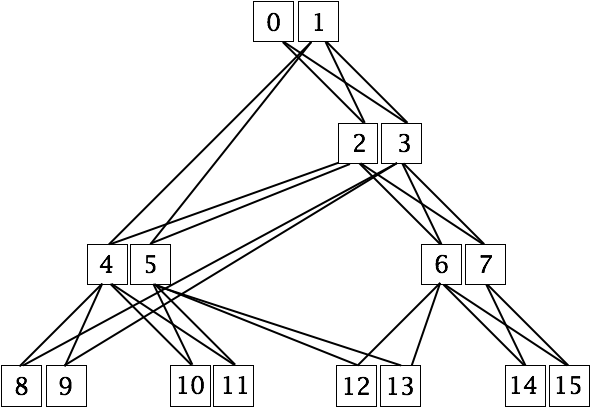
\includegraphics[scale=0.4]{FiguresMaths/FiboFast.png}
        \caption{Dependency relations for computing the pairs $(F(2n),F(2n+1))$.}
                \label{fig:fastFibo}
\end{center}
\end{figure}
In particular, we show how to compute an element ($F(13)$) using the fast Fibonacci scheme in Fig.~\ref{fig:fastFibo13}.
The pattern is embedded into a complete binary tree of predecessors (with some redundancies)
whose depth is logarithmic.
\begin{figure}[h]
\begin{center}
        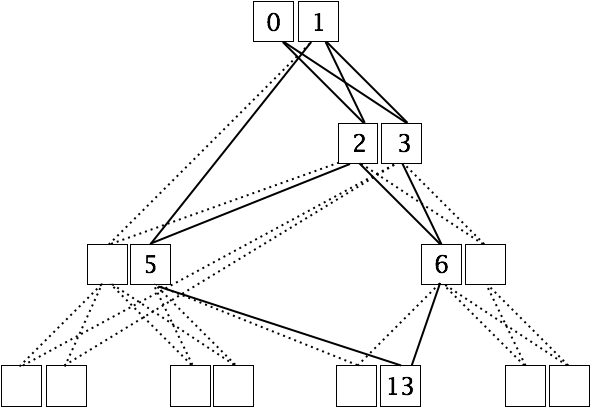
\includegraphics[scale=0.4]{FiguresMaths/FiboFast13.png}
        \caption{Ancestors involved in the computation of $F(13)$. }
        \label{fig:fastFibo13}
\end{center}
\end{figure}

\noindent \textit{Conclusion:}
Any Fibonacci number $F(n)$ can be computed very fast in $log_2 (n)$ steps.


\section{Cassini's identity}

\noindent \textit{The aim:}
Prove a classical identity involving Fibonacci numbers, which is a nice example of proof by recurrence.

\noindent \textit{The problem:}
$F(n-1).F(n+1) = F(n)^2 + (-1)^{n+1}$ for $n \geq 1$
\medskip

%Let check the expression on the first ranks:
%
%$n=1$, $F(0).F(2) = F(1)^2 +1 = 2$
%
%$n=2$, $F(1).F(3) = F(2)^2 -1 = 3$
%
%$n=3$, $F(2).F(4) = F(3)^2 +1 = 10$
%
%$n=4$, $F(3).F(5) = F(4)^2 -1 = 24$
%
%...
%\medskip

\noindent \textit{The solution:}
The proof is by induction.

The basis case $n=1$ holds since $F(0).F(2) = F(1)^2 +1 = 2$.

The induction step is proved assuming the Cassini's identity holds at rank $n$.
Replace $F(n+2)$ by its definition in the expression:
 
$F(n).F(n+2) = F(n) (F(n+1)+F(n)) = F(n)^2 + F(n).F(n+1)$

Then, replace the last term using the recurrence hypothesis:

$F(n)^2 = F(n-1).F(n+1) - (-1)^{n+1} =F(n-1).F(n+1) + (-1)^{n+2} $

Thus,
$F(n).F(n+2) = F(n).F(n+1) + F(n-1).F(n+1) + (-1)^{n+2} = F(n+1) (F(n) + F(n-1)) + (-1)^{n+2}$ 

Apply again the definition of Fibonacci sequence $F(n) + F(n-1) = F(n+1)$, we obtain:

$F(n).F(n+2) = F(n+1)^2 + (-1)^{n+2}$

This concludes the proof. 


\subsection{Lucas' numbers} 

\noindent \textit{The aim:}
Fibonacci progression is the most popular and the most simple Definition of Lucas' numbers

\textbf{Definition:}
Given the two starting numbers $L(0) = 1$ and $L(1) = 3$, 
the other Lucas numbers are obtained by the same progression as Fibonacci: 

$L(n+1) = L(n)+L(n-1)$.
\medskip

In order to gain intuition on this problem, let us compute the first ranks in regard to the classical Fibonacci numbers:
\begin{figure}[htb]
\[
\begin{array}{c||r|r|r|r|r|r|r|r|r|r|r}
{\displaystyle n } & k=0 & k=1 & k=2 & k=3 & k=4 & k=5 &
k=6 & k=7 & k=8 & k=9 & \ldots \\
\hline
F(n) & 1 & 1 &  2  &  3  &   5  &   8  &  13  &  21  & 34  & 55  & \ldots \\
\hline
L(n) & 1 & 3 &  4 &  7  &  11  &  18  &  29 & 47  & 76  & 123 & \ldots \\
\hline
\end{array}
\] 
\caption{Correspondence between Fibonacci and Lucas numbers.}
\label{fig:fiboLucas}
\end{figure}
%
%n: $~~~~0, 1, 2, 3, ~4, ~5, ~6, ~7, ~8, ~~9, ...$
%
%F(n): $1, 1, 2, 3, ~5, ~8, 13, 21, 34, ~55, ...$
%
%L(n): $1, 3, 4, 7, 11, 18, 29, 47, 76, 123, ...$
\medskip

%
%There are strong links with Fibonacci numbers.
%In particular, we established before that
%\bigskip
%
%$F(n+2) = 1+ \sum_{k=0}^{n} F(k)$. 
%\bigskip
%
%We have similarly: $L(n+2) = 1+ \sum_{k=-1}^{n} L(k)$ since the basic step of the induction is still valid: 
%
%$L(2) = L(-1 )+L(0) +1 = 2+1+1 = 4$.
%%Actually, it will be true for all the progressions where $u_1=1$.
%

\noindent \textit{The problem:}
Our purpose is to prove the following expression

$F(k-1).L(n) = F(n+k)+ (-1)^{k-1}F(n-k)$ for $k \leq n$
\bigskip

\noindent \textit{The solution:} 

There are two integers involved here ($k$ and $n$).
Let us study the expression step by step for successive values of $k$.
\medskip

\begin{itemize}
\item Starting smoothly with $k=1$

We can easily show by induction on $n$ that the Lucas number of order $n$ is the sum of two Fibonacci numbers:

$L(n) = F(n-1)+F(n+1)$ for $n \geq 1$
\medskip

%Let check this property on the first ranks:
%
%$n=2$, $L(2) = F(1)+F(3) = 1 + 3 = 4$
%
%$n=3$, $L(3) = F(2)+F(4) = 2 + 5 = 7$
%
%$n=4$, $L(4) = F(3)+F(5) = 3 + 8 = 11$
%
%$n=5$, $L(5) = F(4)+F(6) = 5 + 13 = 18$
%

The basis case, corresponding to for $n=1$) is true since $L(1) = 3 = F(2) + F(0) = 2+1$.

Let assume for proving the induction step that the property holds at all ranks $k \leq n$ and compute $L(n+1)$:

Apply the definition of Lucas' numbers: $L(n+1) = L(n)+L(n-1)$

Apply the induction hypothesis on both terms of the right hand side:

 $L(n+1) = F(n+1)+F(n-1)+F(n)+F(n-2)$

Apply now the definition of Fibonacci numbers for $F(n+1) + F(n) = F(n+2)$  and $F(n-1) + F(n-2) = F(n)$

Replace them in the previous expression:

$L(n+1) = F(n+2)+F(n)$

which concludes the proof.

\item
Extension.

Using a similar approach, we obtain $L(n) = F(n+2)-F(n-2)$. 
What happens if we generalize? Easy calculations lead to the following results:
\medskip

$2.L(n) = F(n+3) + F(n-3) $

%Proposition.
%
%$2.L(n) = F(n+3)+F(n-3)$
%\bigskip
%
%Proof.
%We start from $L(n) = F(n+2)-F(n-2)$
%
%$F(n+2) = F(n+3) - F(n+1)$ and $F(n-2) = F(n-1) - F(n-3)$
%
%$L(n) = F(n+3) - (F(n+1) + F(n-1)) + F(n-3)$
%
%$2.L(n) = F(n+3) + F(n-3)$
%
%
%\item Extension 2
%
%Go to the next step using the same technique:
%\medskip
%
%
%
%$= F(n+4) - F(n+2) + F(n-2) - F(n-4)$
%\medskip

$3.L(n) = F(n+4) - F(n-4)$

$5.L(n) = F(n+5) + F(n-5)$
\medskip
 
As $2, 3, 5$ are successive Fibonacci numbers, this gives us the intuition of the general case:

$F(k-1).L(n) = F(n+k) + (-1)^{k-1}F(n-k)$ for $k \leq n$
\medskip

which is proved (again) as follows by induction assuming the expression holds at rank up to $k$.

The basis case is straightforward (see case $k=1$).

Compute $F((k+1)-1).L(n)$ and apply the definition of Fibonacci number $F((k+1)-1) = F(k-1) + F(k-2)$

$F(k).L(n) = F(k-1).L(n + F(k-2).L(n)$ and replace both last terms by using the induction hypothesis:

$= F(n+k) + (-1)^{k-1}F(n-k) + F(n+k-1) + (-1)^{k-2}F(n-(k-1))$

$= F(n+k) +  F(n+k-1) + (-1)^{k-1}(F(n-k) - F(n-k+1))$

The final result is obtained by applying twice the definition of the Fibonacci numbers.


\end{itemize}
